\documentclass{beamer}

\usepackage[utf8]{inputenc} \usepackage[T1]{fontenc} \usepackage[ngerman]{babel} \usepackage[nice]{nicefrac} 
\usepackage{amsmath, amsfonts, amssymb, mathptmx, microtype, booktabs, graphicx, wrapfig, float, color, ulem, multimedia}
%\usepackage[unicode]{hyperref}

\usetheme{Warsaw}
\title[Optisches Pumpen]{OPTISCHES PUMPEN \\ Kernspinmessung mit dem Kompass}
\author{Robi Pedersen und Simon Schmeißer}
\institute{Albert-Ludwigs-Universität Freiburg}
\date{23. März 2011}

\begin{document}

\begin{frame}
\titlepage
\end{frame}

\begin{frame}[shrink]{Inhalt}
\tableofcontents
\end{frame}

%------------------------------------------------------------------------------------------------------------------------------------------------

\section{Einleitung}

\begin{frame}{Aufgabenstellung} %eventuell kürzer
\begin{itemize}
\item Hyperfeinstrukturspektrum des $^2S_{1/2} - ^2P_{1/2}$-Übergangs von $^{85}Rb$ und $^{87}Rb$.
\item Kernspin der Rubidium-Isotope anhand Doppelresonanz.
\item Bestimmen der Horizontal- und Vertikalkomponente des Erdmagnetfelds. 
\item Spinpräzession von ausgerichteten Atomen um das Erdmagnetfeld.
\item Relaxationszeit nach Dehmelt und nach Franzen. 
\end{itemize}
\end{frame}

%-------------------------------------------------------------

\subsection{Was ist optisches Pumpen?}

\begin{frame}{Was ist optisches Pumpen?}
Erfinder: Alfred Kastler 1950 (Nobelpreis 1966)
	\begin{figure}[H]
	\movie[poster, height = 4.5 cm, width = 10 cm]{Feinstrukturpumpen}{Movies/animation2.flv}
	\caption{Feinstrukturpumpen}
	\end{figure}
\end{frame}


\begin{frame}{Was ist optisches Pumpen?}
Erfinder: Alfred Kastler 1950 (Nobelpreis 1966)
\begin{columns}
\begin{column}{5cm}
	\begin{figure}[H]
	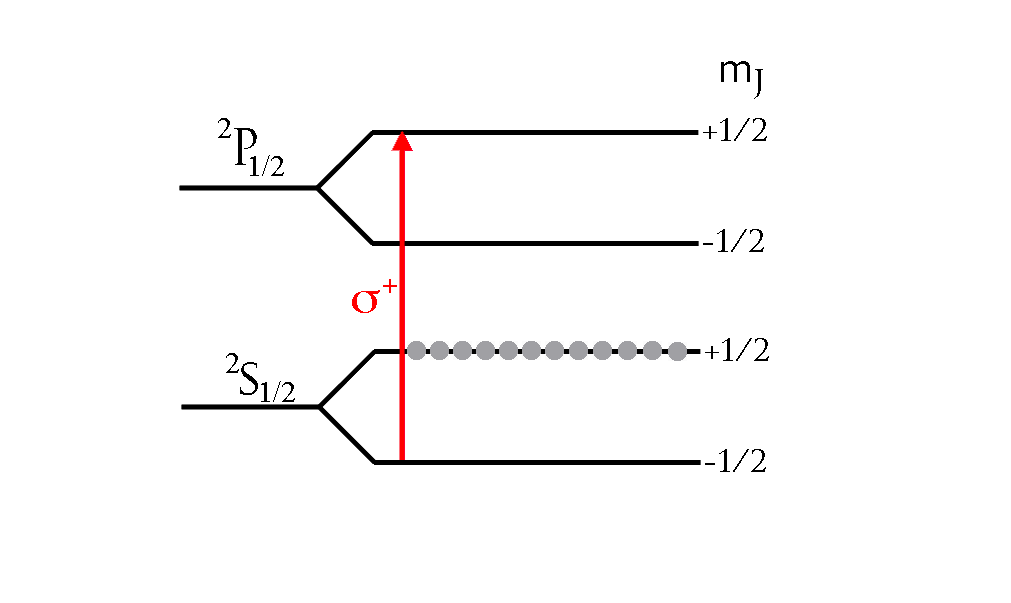
\includegraphics[width = \textwidth]{Movies/animation2197.png}
	\caption{Feinstrukturpumpen}
	\end{figure}
\end{column}
\begin{column}{5cm}
	\begin{itemize}
	 \item Laser
	 \item Resonanzspektroskopie
	 \item Kernspinbestimmung
	 \item Hyperfeinstrukturintervalle
	 \item Landé g-Faktoren
	 \item Erdmagnetfeld
	\end{itemize}
\end{column}
\end{columns}
\end{frame}


\section{Laserkennlinie} %----------------------------------------------------

\subsection{Die Laserdiode}

\begin{frame}
\begin{center}
\centering {\LARGE Die Laserkennlinie}
\end{center}
\end{frame}

\begin{frame}{Die Halbleiter-Laserdiode} 
\begin{figure}
 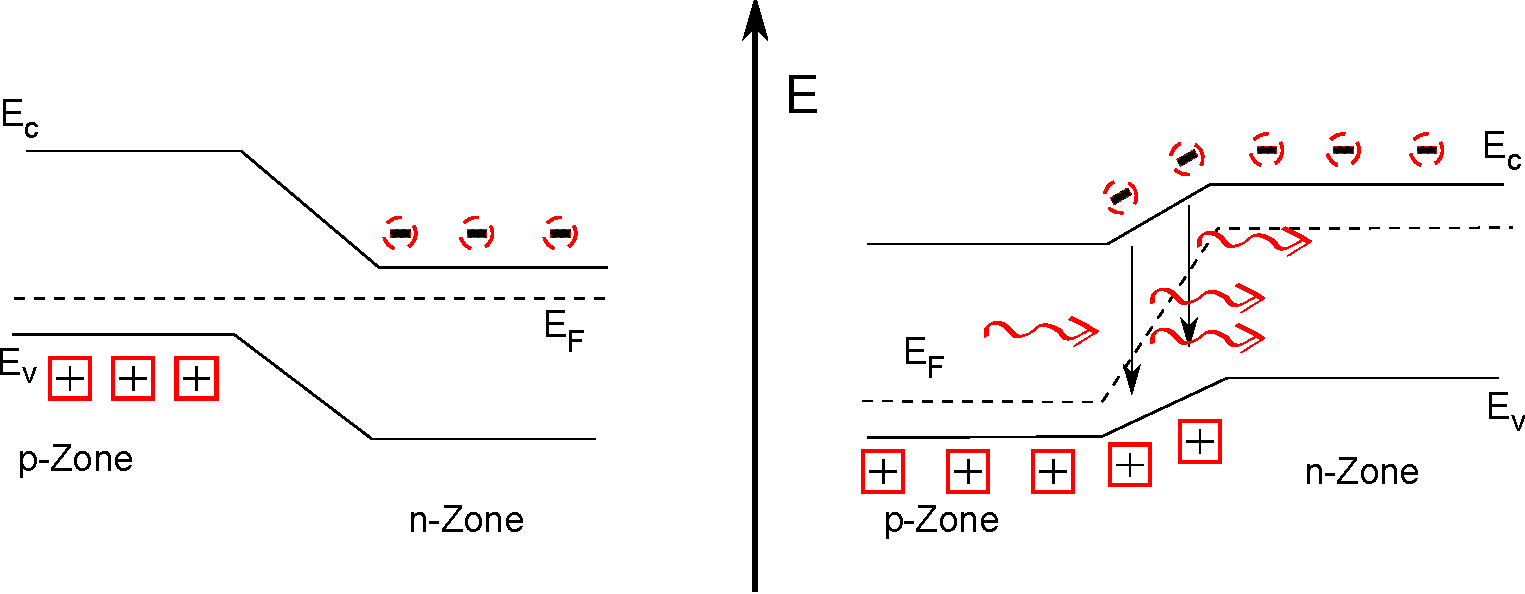
\includegraphics[width=\textwidth]{Bilder/p-n.pdf}
\end{figure}

\end{frame}

\subsection{Der Versuchsaufbau}
\begin{frame}{Der Versuch}
\centering 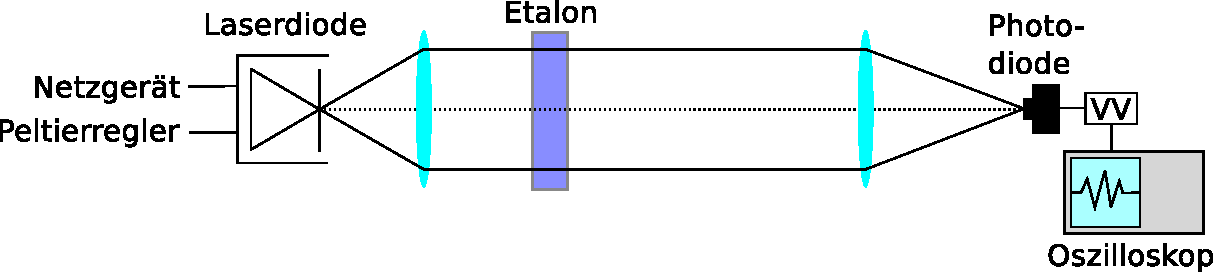
\includegraphics[width=\textwidth]{Bilder/ABLaser.pdf}
\begin{columns}
\begin{column}{4cm}
\pause \centering 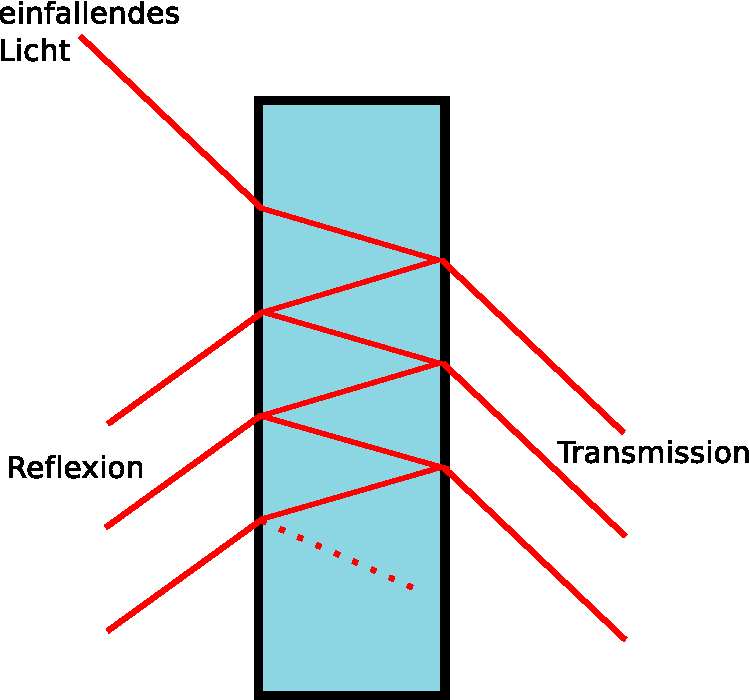
\includegraphics[width=\textwidth]{Bilder/etalon.pdf}
\end{column}
\begin{column}{5cm}
Distanz der Maxima
$$ FSR = (9924 \pm 30) MHz $$
\end{column}
\end{columns}
\end{frame}

\subsection{Ergebnisse}
\begin{frame}{Wandern der Maxima}
\begin{columns}
\begin{column}{5cm}
	\begin{figure}[H]
	\movie[poster, height = 3.5 cm, width = 4.8 cm]{Wandern der Maxima}{Movies/I-aendert.AVI}
	\caption{Veränderung des Stroms}
	\end{figure}
\end{column}
\begin{column}{5cm}
	\begin{figure}[H]
	\movie[poster, height = 3.5 cm, width = 4.8 cm]{Wandern der Maxima}{Movies/T-aendert.AVI}
	\caption{Veränderung der Temperatur}
	\end{figure}
\end{column}
\end{columns}
\end{frame}

\begin{frame}{Messergebnisse}
\begin{columns}
\begin{column}{5cm}
	\begin{figure}[H]
	\centering 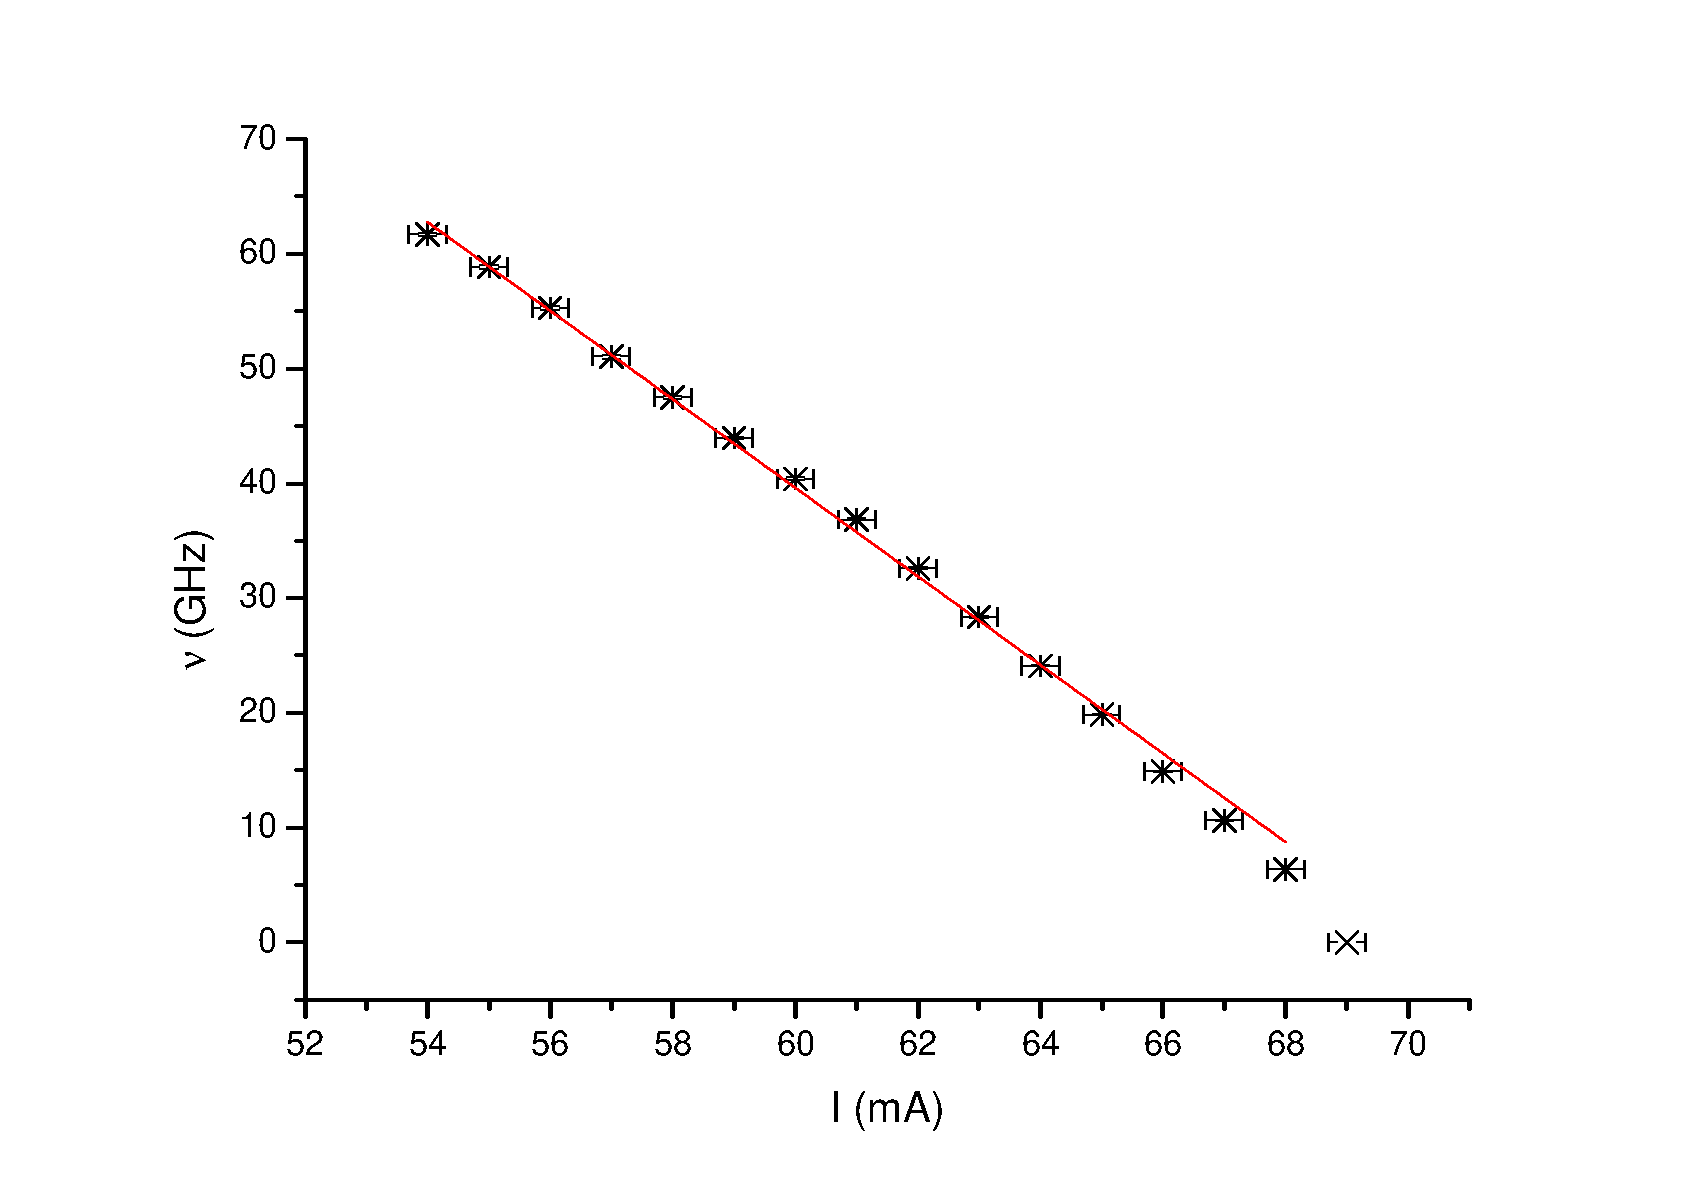
\includegraphics[width=1\textwidth]{Bilder/T_fest.pdf}
	\caption{Veränderung des Stroms}
	\end{figure}
\end{column}
\begin{column}{5cm}
	\begin{figure}[H]
	\centering 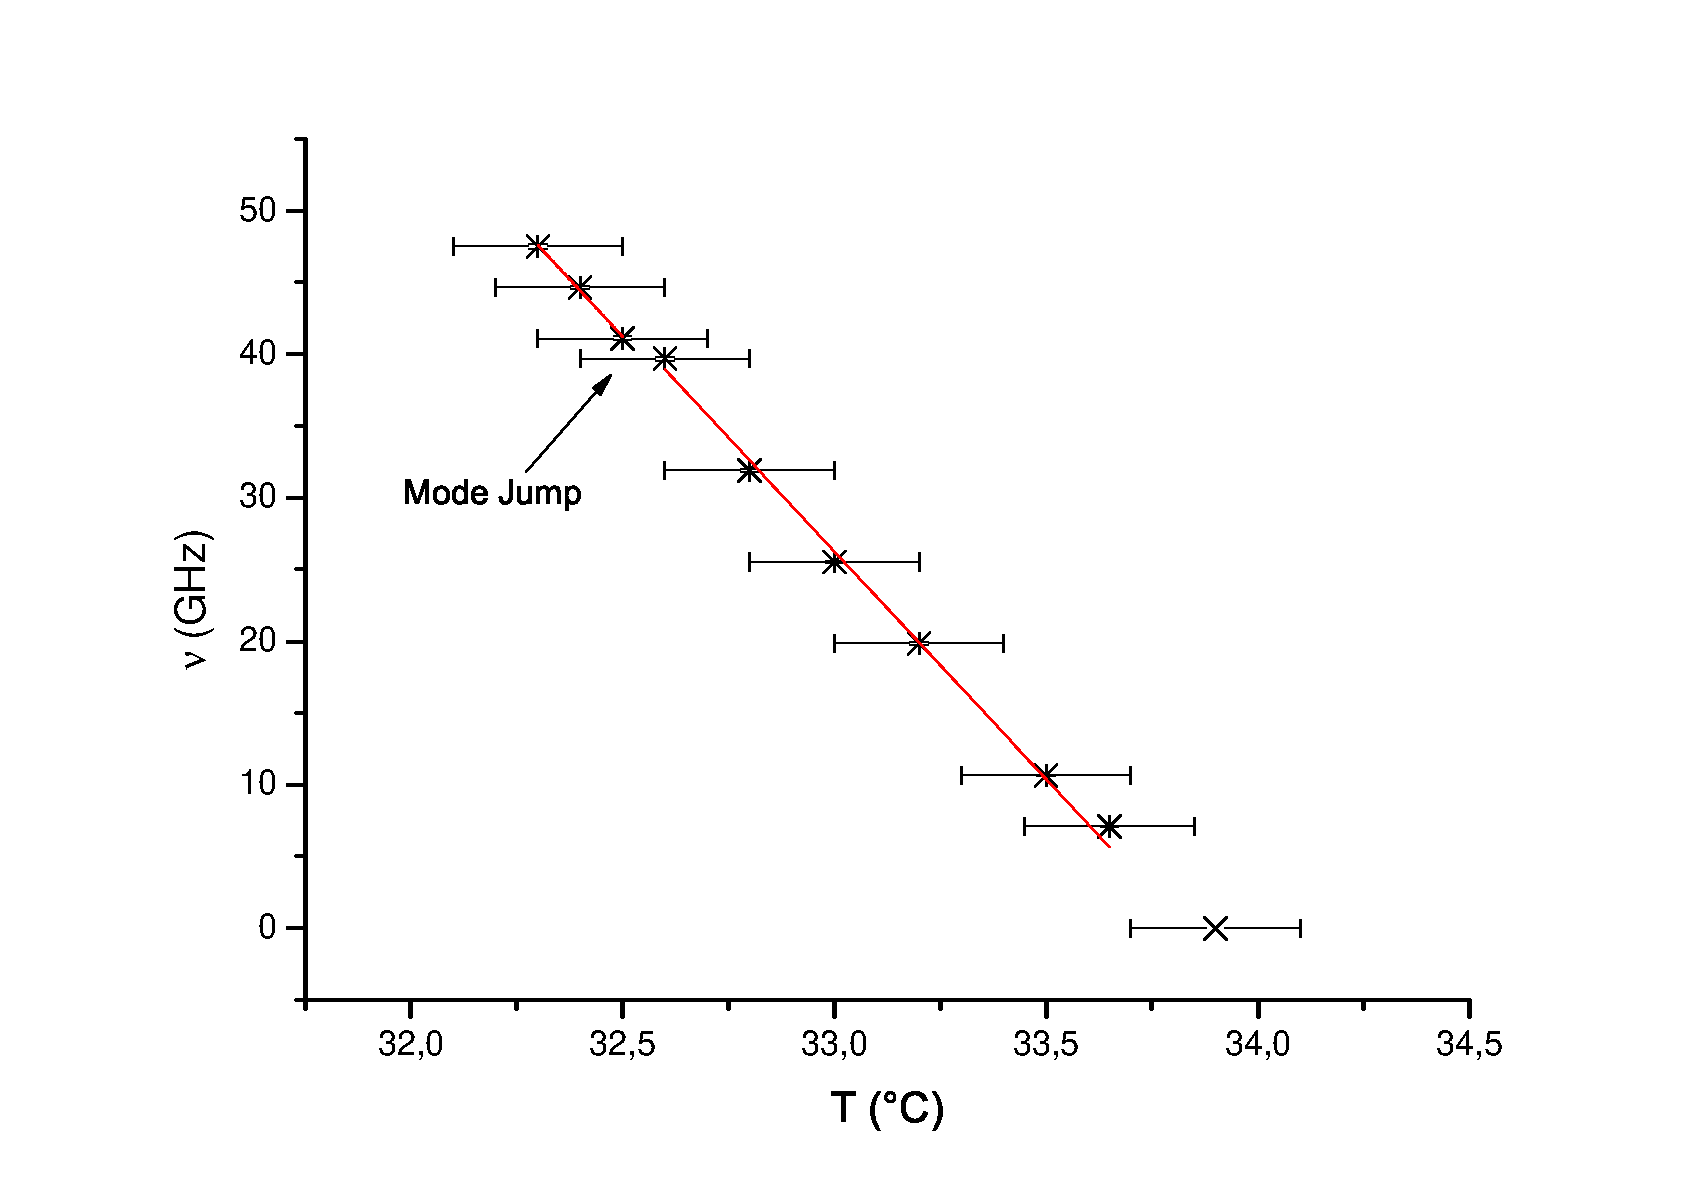
\includegraphics[width=1\textwidth]{Bilder/I_fest.pdf}
	\caption{Veränderung der Temperatur}
	\end{figure}
\end{column}
\end{columns}
$$\Delta\nu = (-3.86 \pm 0.06)\Delta I GHz/ma$$
$$\Delta\nu = (-31.70 \pm 1.12)\Delta I GHz/^\circ C$$
\end{frame}


\section{Die Hyperfeinstruktur}

\begin{frame}
\begin{center}
\centering {\LARGE Die Hyperfeinstruktur}
\end{center}
\end{frame}


\subsection{Theorie}
\begin{frame}{Feinstruktur}
\begin{columns}
\begin{column}{4.5cm}
	\begin{figure}[H]
	\centering 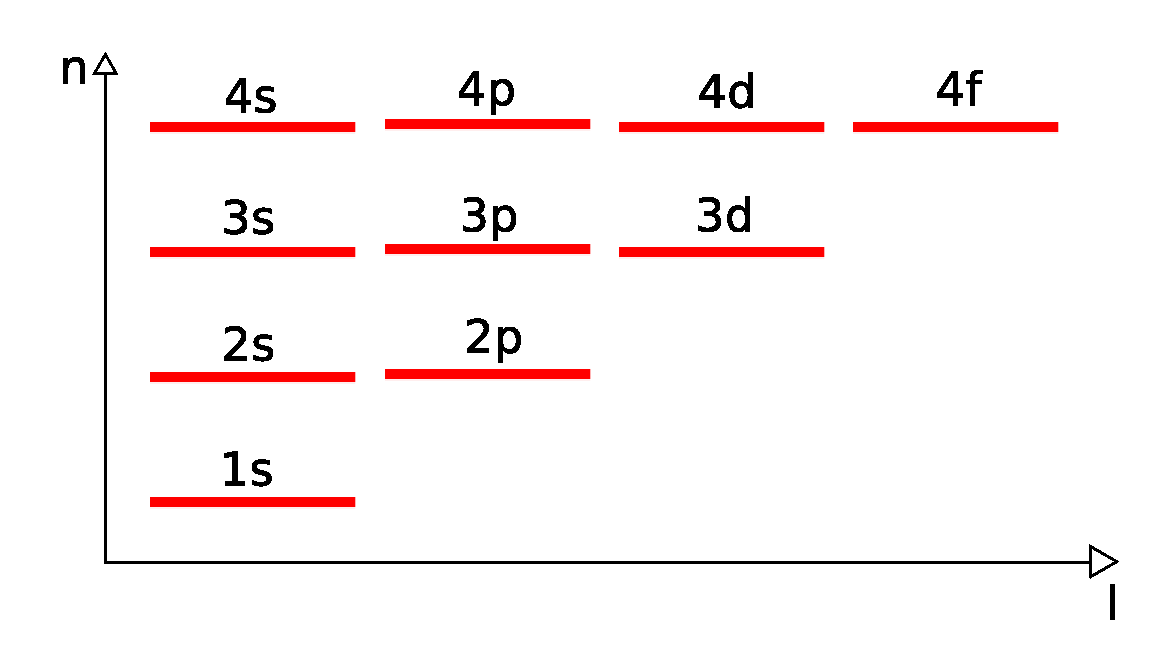
\includegraphics[width=1.2\textwidth]{Bilder/bohrspektrum.pdf}
	\caption{Klassische Energieniveaus}
	\end{figure} %blabla entartet
\end{column}
\begin{column}{5.5cm}
\pause Feinstruktur:
\begin{itemize}
	\item Elektronenspin $\vec S$
	\item Spin-Bahn-Kopplung, Drehimpuls $\vec J = \vec L + \vec S$
\end{itemize}
\end{column}
\end{columns}
\end{frame}


\begin{frame}{Feinstruktur}
\begin{columns}
\begin{column}{4.5cm}
	\begin{figure}[H]
	\centering 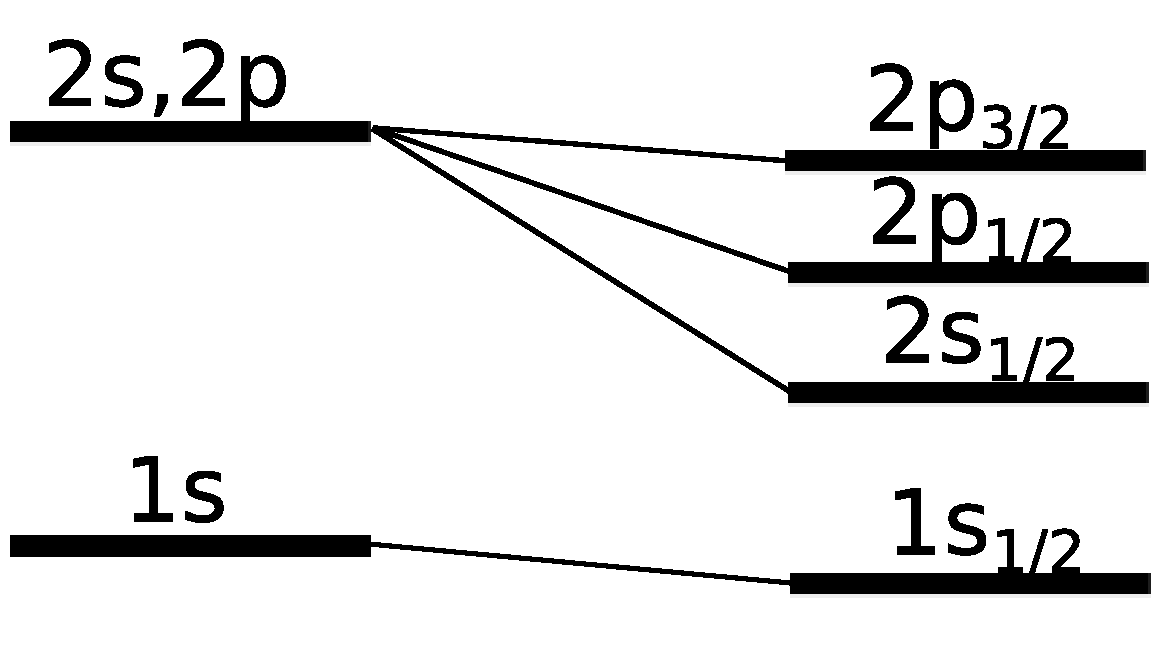
\includegraphics[width=\textwidth]{Bilder/feinstruktur.pdf}
	\caption{Feinstruktur-Energieniveaus}
	\end{figure}
\end{column}
\begin{column}{5.5cm}
Feinstruktur:
\begin{itemize}
	\item Elektronenspin $\vec S$
	\item Spin-Bahn-Kopplung, Gesamtdrehimpuls $\vec J = \vec L + \vec S$
	\item Magnetisches Moment $\vec\mu_J$
	\item Aufspaltung der Energieniveaus
	\item Aufhebung der Entartung
\end{itemize}
\end{column}
\end{columns}
\end{frame}


\begin{frame}{Hyperfeinstruktur}
\begin{itemize}
\item Kernspin $\vec I$
\item Drehimpulskopplung, Gesamtdrehimpuls $\vec F = \vec I + \vec J$
\item Magnetisches Moment des Kerns $$\vec \mu_I = \frac{g_I\mu_K}{\hbar} \vec I $$
\item Aufspaltung der Energieniveaus $$E_{HFS} = -\vec\mu_I\vec B_J$$
\end{itemize}
\end{frame}


\begin{frame}{Hyperfeinstruktur}
\begin{columns}
\begin{column}{4.5cm}
	\begin{figure}[H]
	\centering 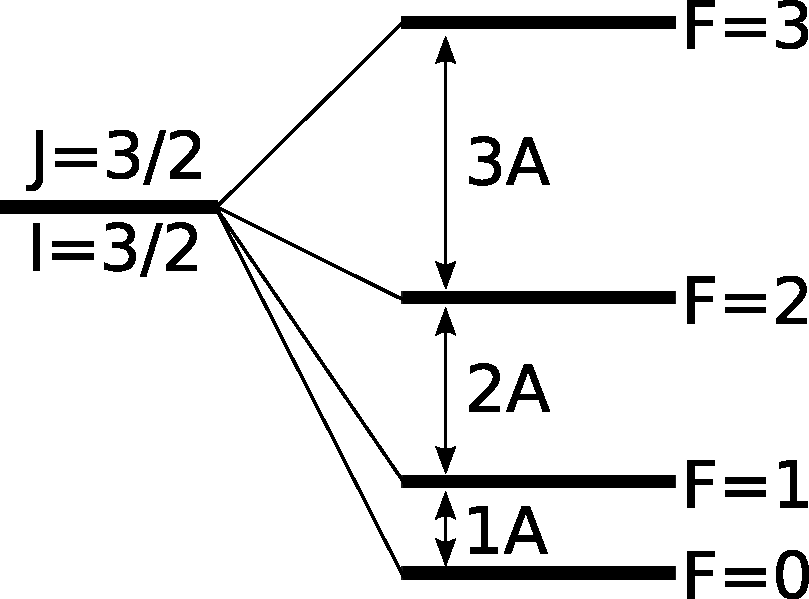
\includegraphics[width=\textwidth]{Bilder/hfstheo.pdf}
	\caption{Feinstruktur-Energieniveaus}
	\end{figure}
\end{column}
\begin{column}{5.5cm}
Differenz zwischen zwei benachbarten Zuständen:

$$\Delta E_{\Delta F = 1} = A(F+1)$$

Hyperfein-Intervallkonstante

$$ A = \frac{g_I\mu_KB_J}{\sqrt{J(J+1)}} $$

\end{column}
\end{columns}
\end{frame}


\begin{frame}{Der Zeeman-Effekt}
\begin{columns}
\begin{column}{4.5cm}
	\begin{figure}[H]
	\centering 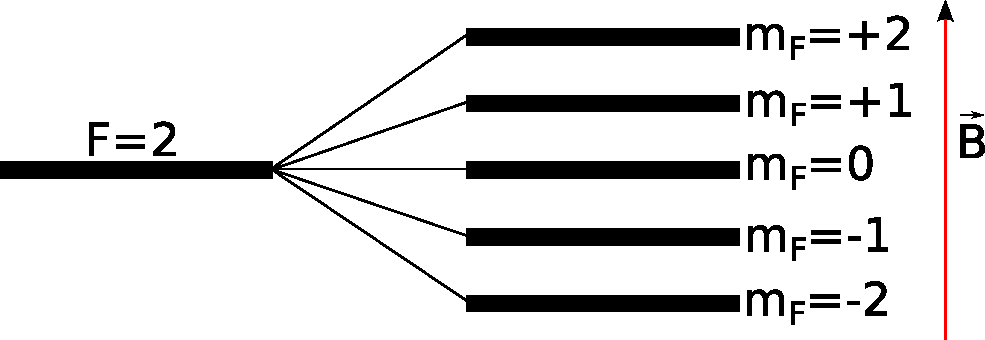
\includegraphics[width=\textwidth]{Bilder/Zeeman.pdf}
	\caption{Zeeman-Aufspaltung von F=2}
	\end{figure}
\end{column}
\begin{column}{5.5cm}
Externes Magnetfeld $\vec B$ \\ $\Rightarrow$ Aufhebung der Entartung in 2F+1 Zustände: $m_F = -2,\dots,+2$
$$E_{Aufspaltung} = - \vec\mu_F\vec B$$ 
$$\vec\mu_F = \vec\mu_I + \vec \mu_J$$

Für J=1/2:

$$\Delta E_{\Delta m_F=1} = \frac{g_J}{2I+1}\mu_B B$$
\end{column}
\end{columns}
\end{frame}


\subsection{Hyperfeinstrukturspektrum}
\begin{frame}{Das Hyperfeinstrukturspektrum von Rubidium}
	\begin{figure}[H]
	\centering 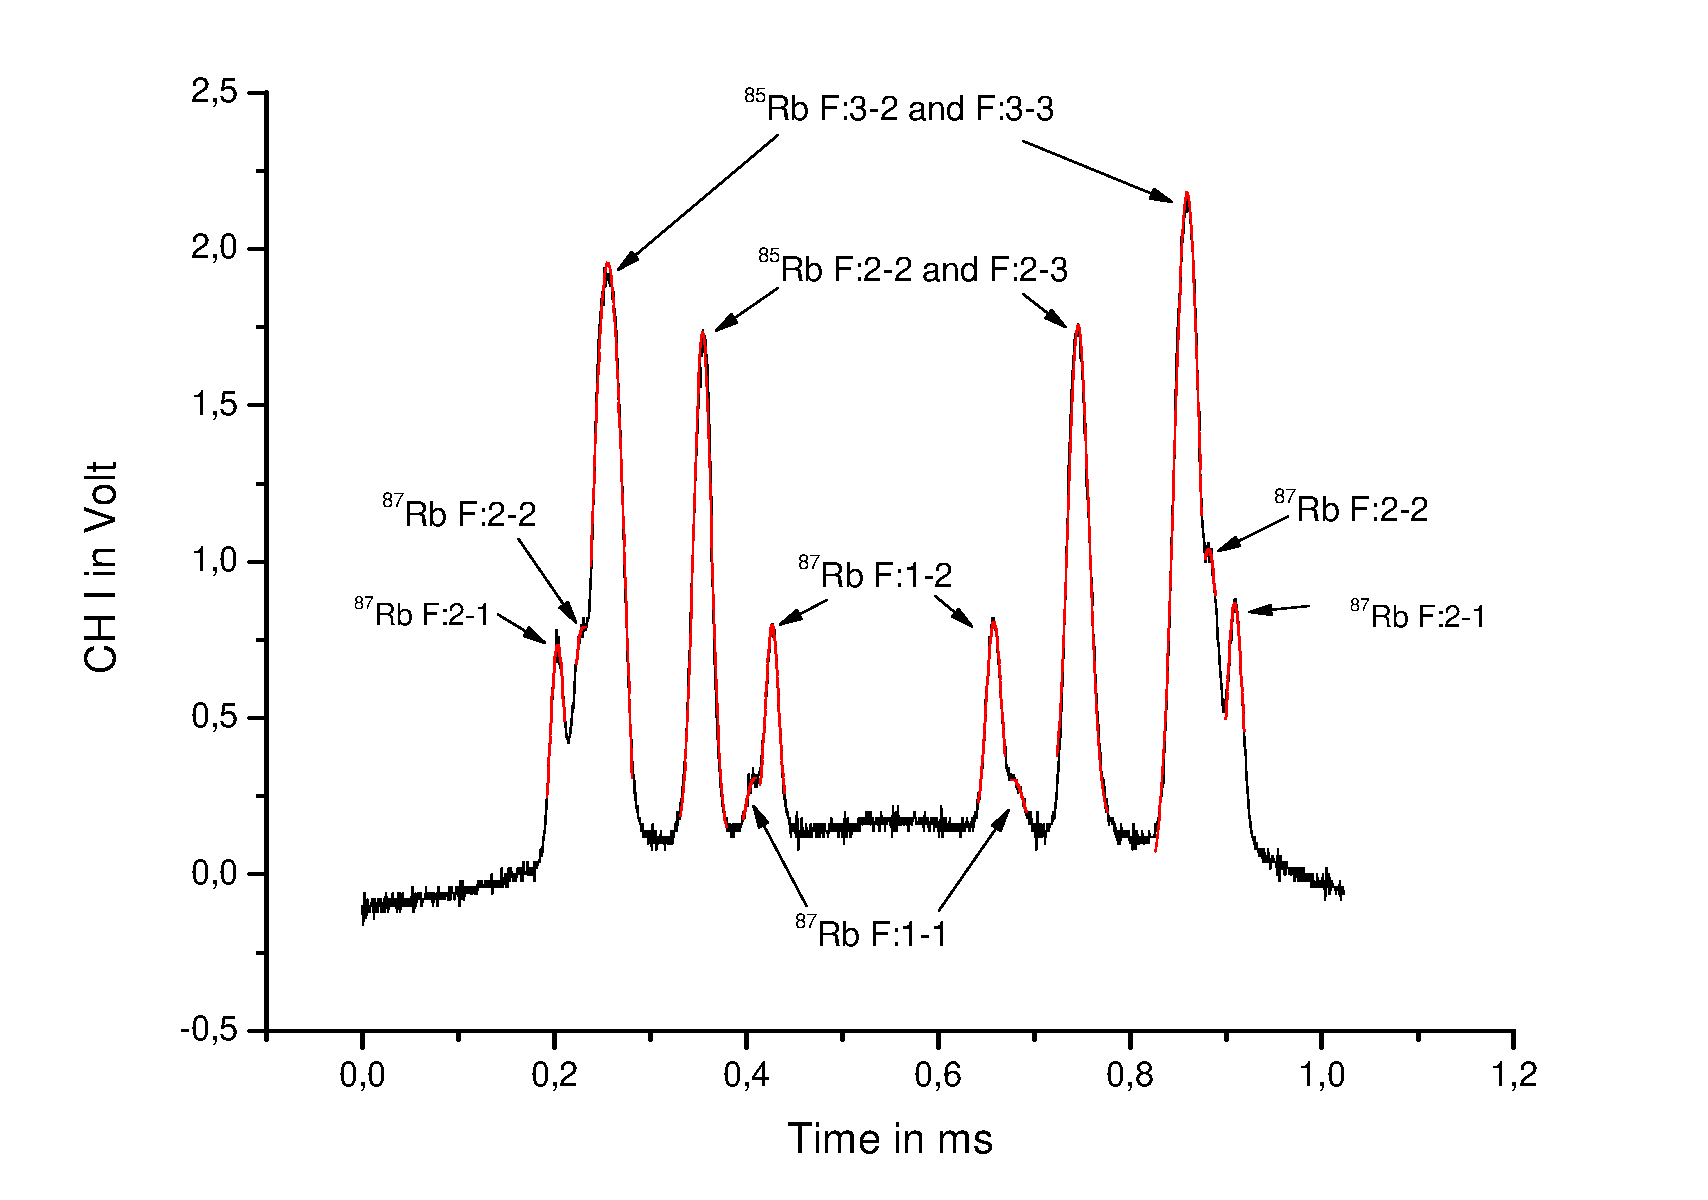
\includegraphics[width=0.94\textwidth]{Bilder/HFS.pdf}
	\end{figure}
\end{frame}

\subsection{Messung}
\begin{frame}{Der Versuchsaufbau}
	\centering 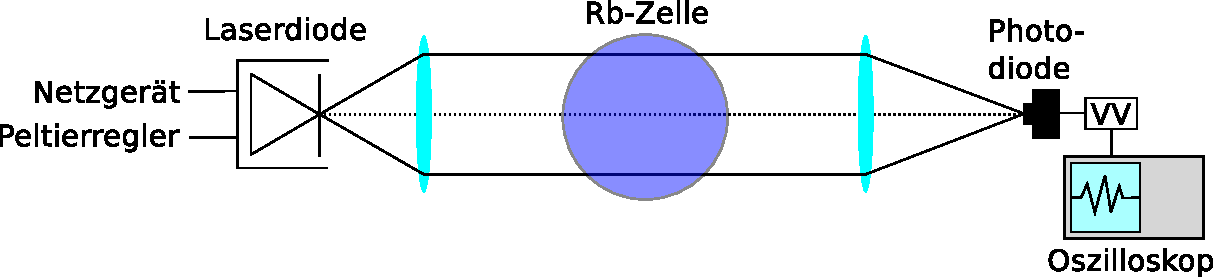
\includegraphics[width=1\textwidth]{Bilder/ABHFS.pdf}
	\begin{block}{Die Rubidium-Zelle}
	\begin{itemize}
	\item $^{87}Rb$ (27.2\%) und $^{85}Rb$ (72.8\%)
	\item Puffergas: Krypton
	\item Druck: p = 150 Pa
	\end{itemize}
	\end{block}
\end{frame}

\begin{frame}{Die Hyperfeinstruktur von Rubidium}
	\begin{figure}[H]
	\centering 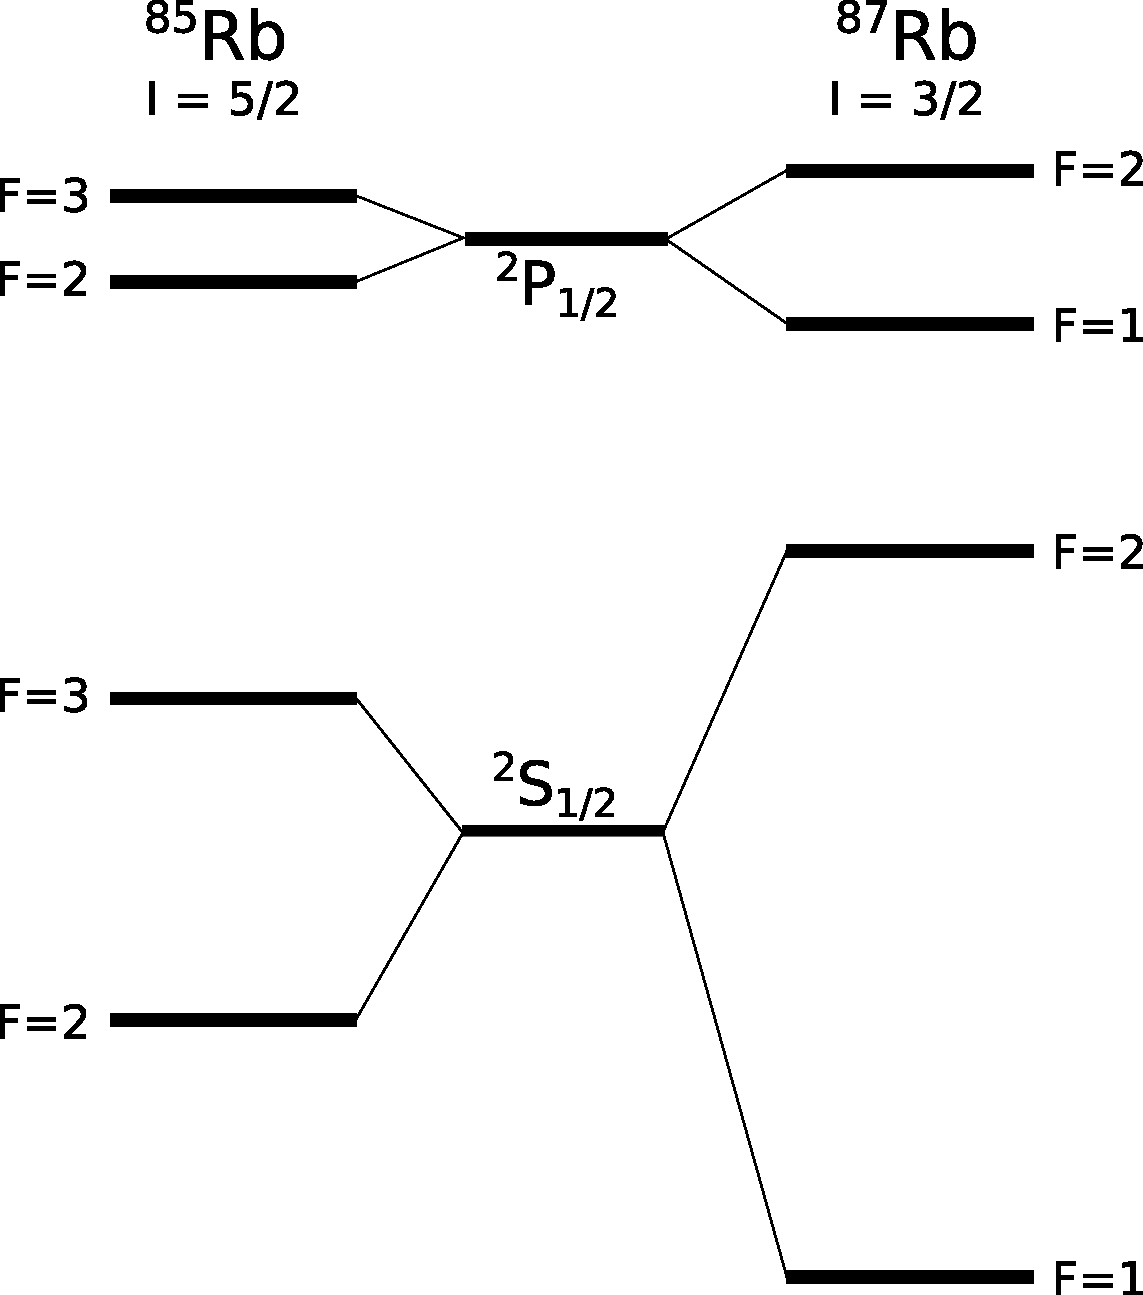
\includegraphics[width=0.5\textwidth]{Bilder/HFSRb.pdf}
	\caption{HFS von Rubidium}
	\end{figure}
\end{frame}

\begin{frame}{Gemessenene Absorptionslinien}
	\begin{figure}[H]
	\centering 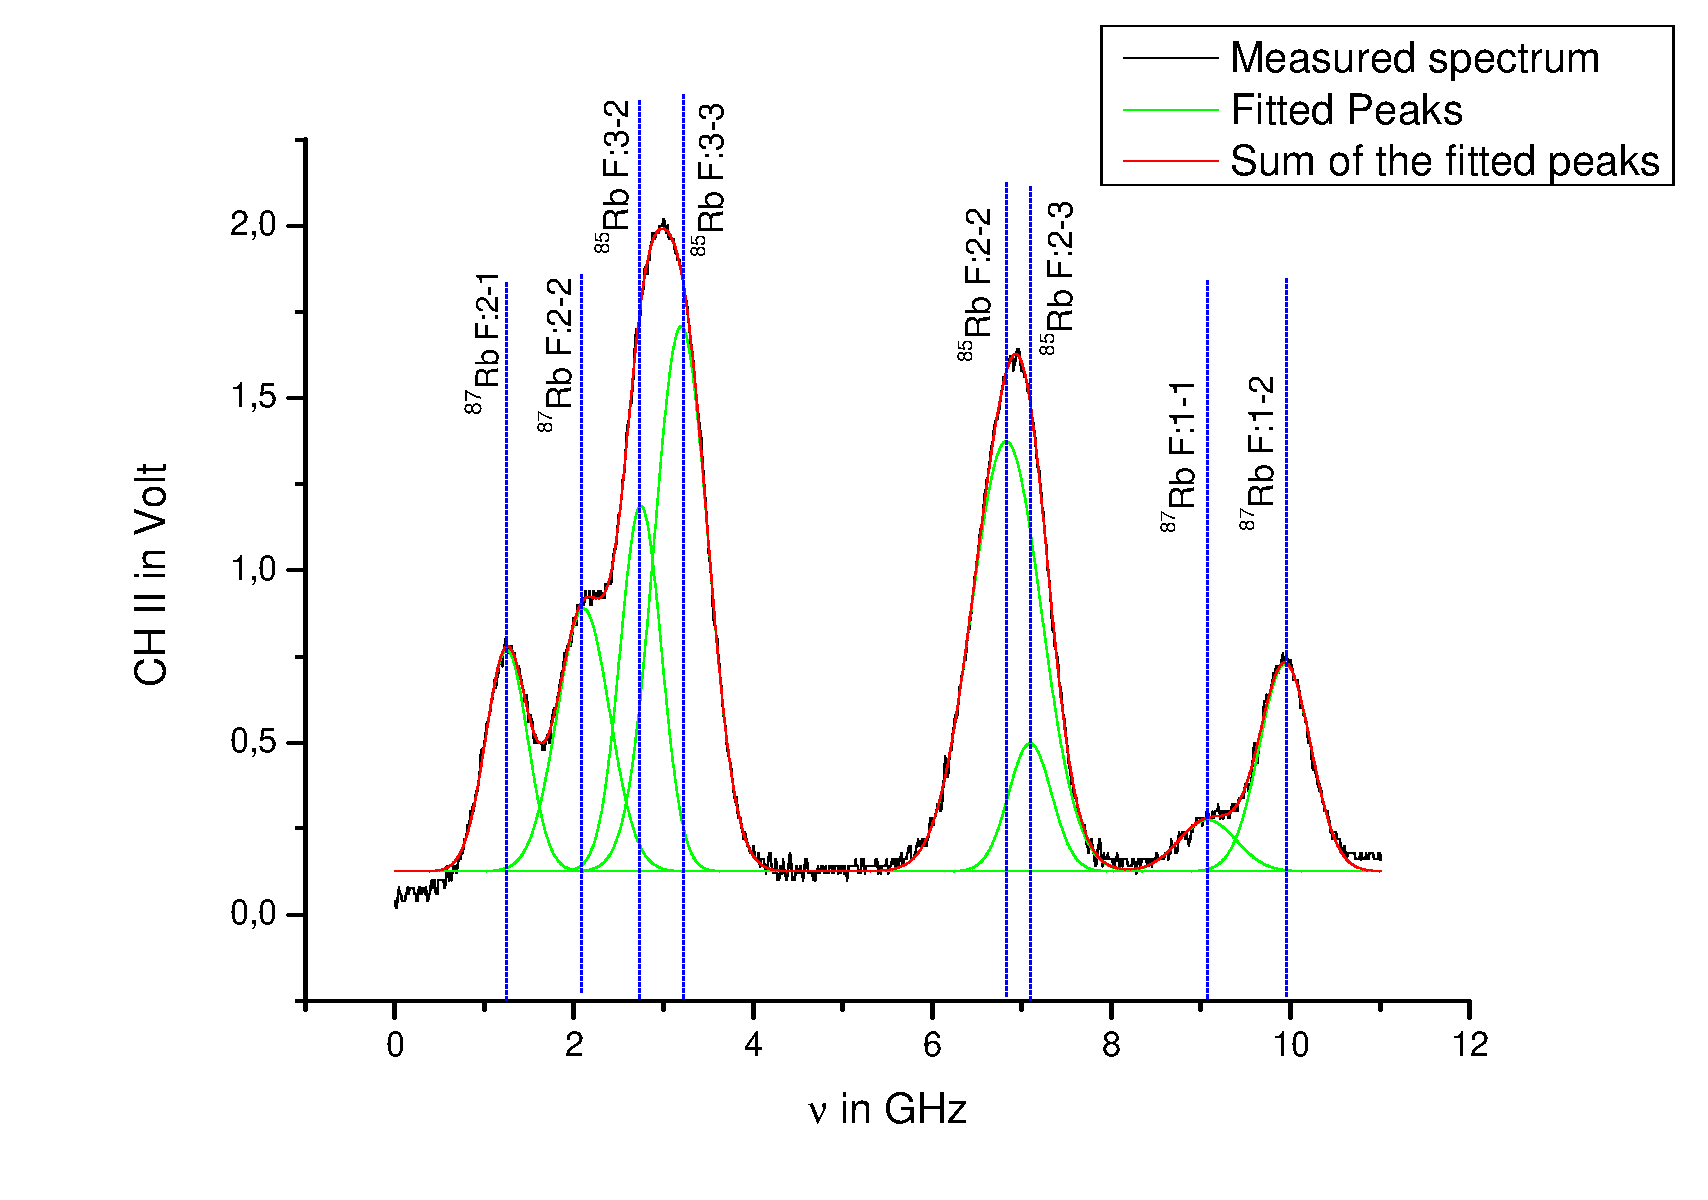
\includegraphics[width=0.95\textwidth]{Bilder/HFSAusw.pdf}
	\end{figure}
\end{frame}

\begin{frame}{Die Intervallkonstanten}

$$A = \frac{\Delta\nu\cdot h}{F+1}$$

\begin{center}
\begin{tabular}[H]{| c | c c c c |} \hline
Isotop & $A_1$ in $\mu$eV & $A_2$ in $\mu$eV & $A_{th.}$ in $\mu$eV & St.-Abw.\\ \hline
$^{87}Rb$, $^2S_{1/2}$ & $16.19 \pm 0.51$ & $16.20 \pm 0.51$ & 14.13  & 5 \\
$^{87}Rb$, $^2P_{1/2}$ & $1.79 \pm 0.51$ &  $1.77 \pm 0.50$ & 1.692   & 1 \\
$^{85}Rb$, $^2S_{1/2}$ & $5.63 \pm 0.33$ &  $5.37 \pm 0.34$ & 4.185   & 4 - 5 \\
$^{85}Rb$, $^2P_{1/2}$ & $0.37 \pm 0.34$ &  $0.62 \pm 0.33$ & 0.499   & 1 \\ \hline
\end{tabular}\\
\end{center}

\end{frame}


\section{Doppelresonanz}
\begin{frame}
\begin{center}
\centering {\LARGE Die Doppelresonanz}
\end{center}
\end{frame}

\subsection{Optisches Pumpen}
\begin{frame}{Stahlungsübergänge}
	\begin{figure}[H]
	\centering 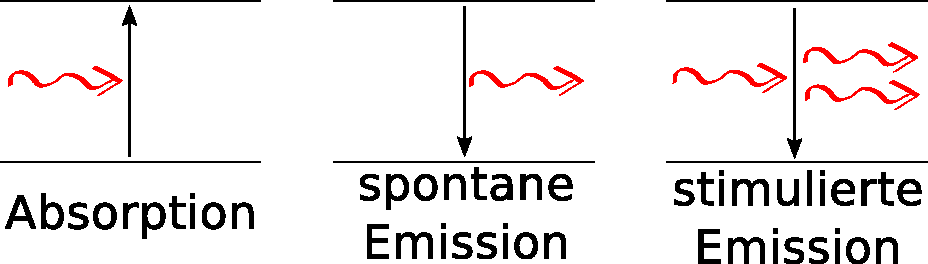
\includegraphics[width=0.95\textwidth]{Bilder/Strahlungsuebergaenge.pdf}
	\end{figure}
\begin{block}{Auswahlregeln für Dipolübergänge}
\begin{center}
\begin{tabular}{l c l}
$\Delta J = 0, \pm 1$ & \, \, \, \, \, \, & $J=0 \not\to J'=0$\\
$\Delta m_J = 0, \pm 1$ &  \, \, \, \, \, \,  & $P \neq P'$ (Parität)\\
\end{tabular}
\end{center}
\end{block}
\end{frame}

\begin{frame}{Optisches Pumpen}
\begin{center}
\begin{tabular}{| c c c |} \hline
$\sigma^-$-Licht 	& \,\,\,\,	$\pi$-Licht \,\,\,\,	 	&	\alert{$\sigma^+$-Licht} 	\\
$\Delta m_J = -1$	& \,\,\,\,	$\Delta m_J = 0$ \,\,\,\,	&	\alert{$\Delta m_J = +1$}	\\ \hline
\end{tabular}
\end{center}
	\begin{figure}[H]
	\centering 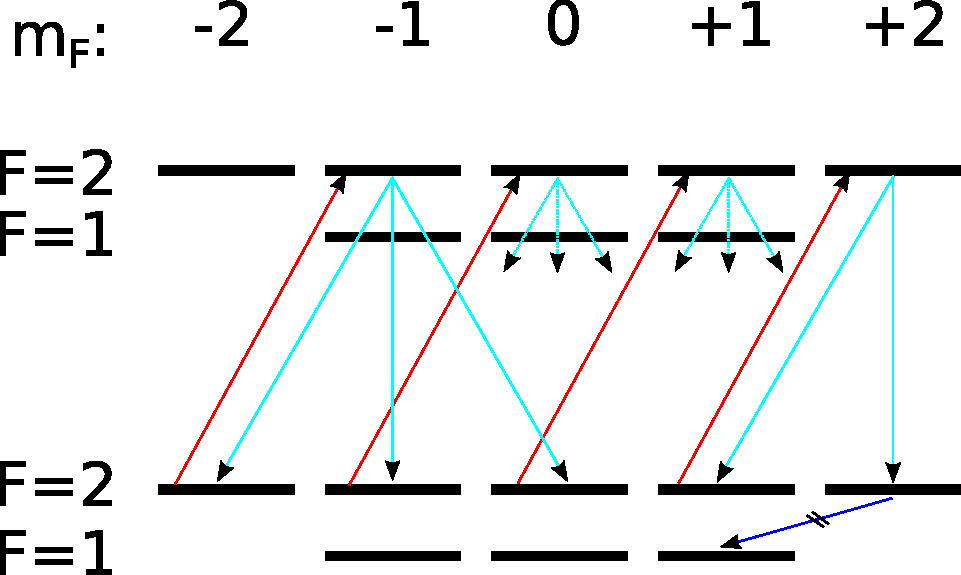
\includegraphics[width=0.7\textwidth]{Bilder/OP87Rb.pdf}
	\end{figure}
\end{frame}

\subsection{Versuchsaufbau}
\begin{frame}{Versuchsaufbau}
	\centering 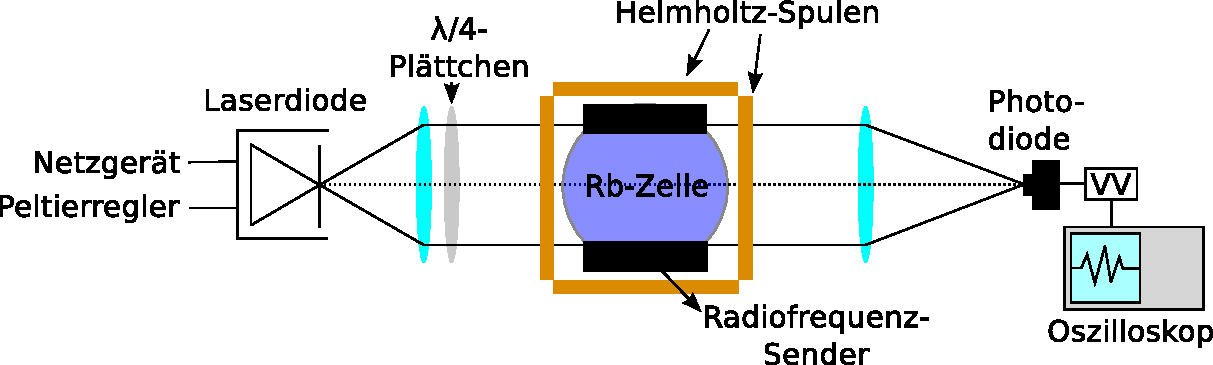
\includegraphics[width=\textwidth]{Bilder/ABDR.pdf}
\end{frame}

\subsection{Prinzip}
\begin{frame}{Prinzip der Doppelresonanz}
\begin{columns}
\begin{column}{3.5cm}
	\begin{figure}[H]
	\centering 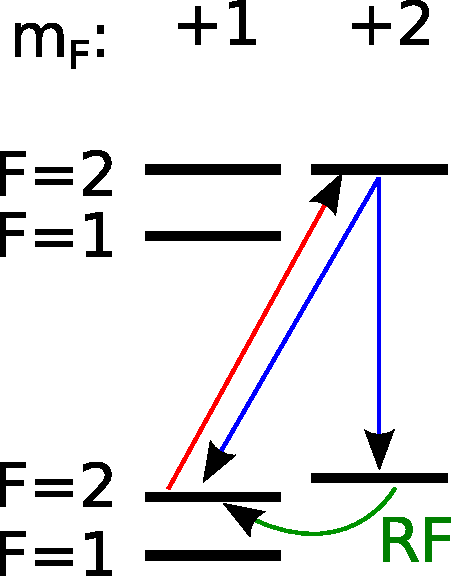
\includegraphics[width=\textwidth]{Bilder/OPRF.pdf}
	\end{figure}
\end{column}
\begin{column}{6.5cm}
\pause \centering 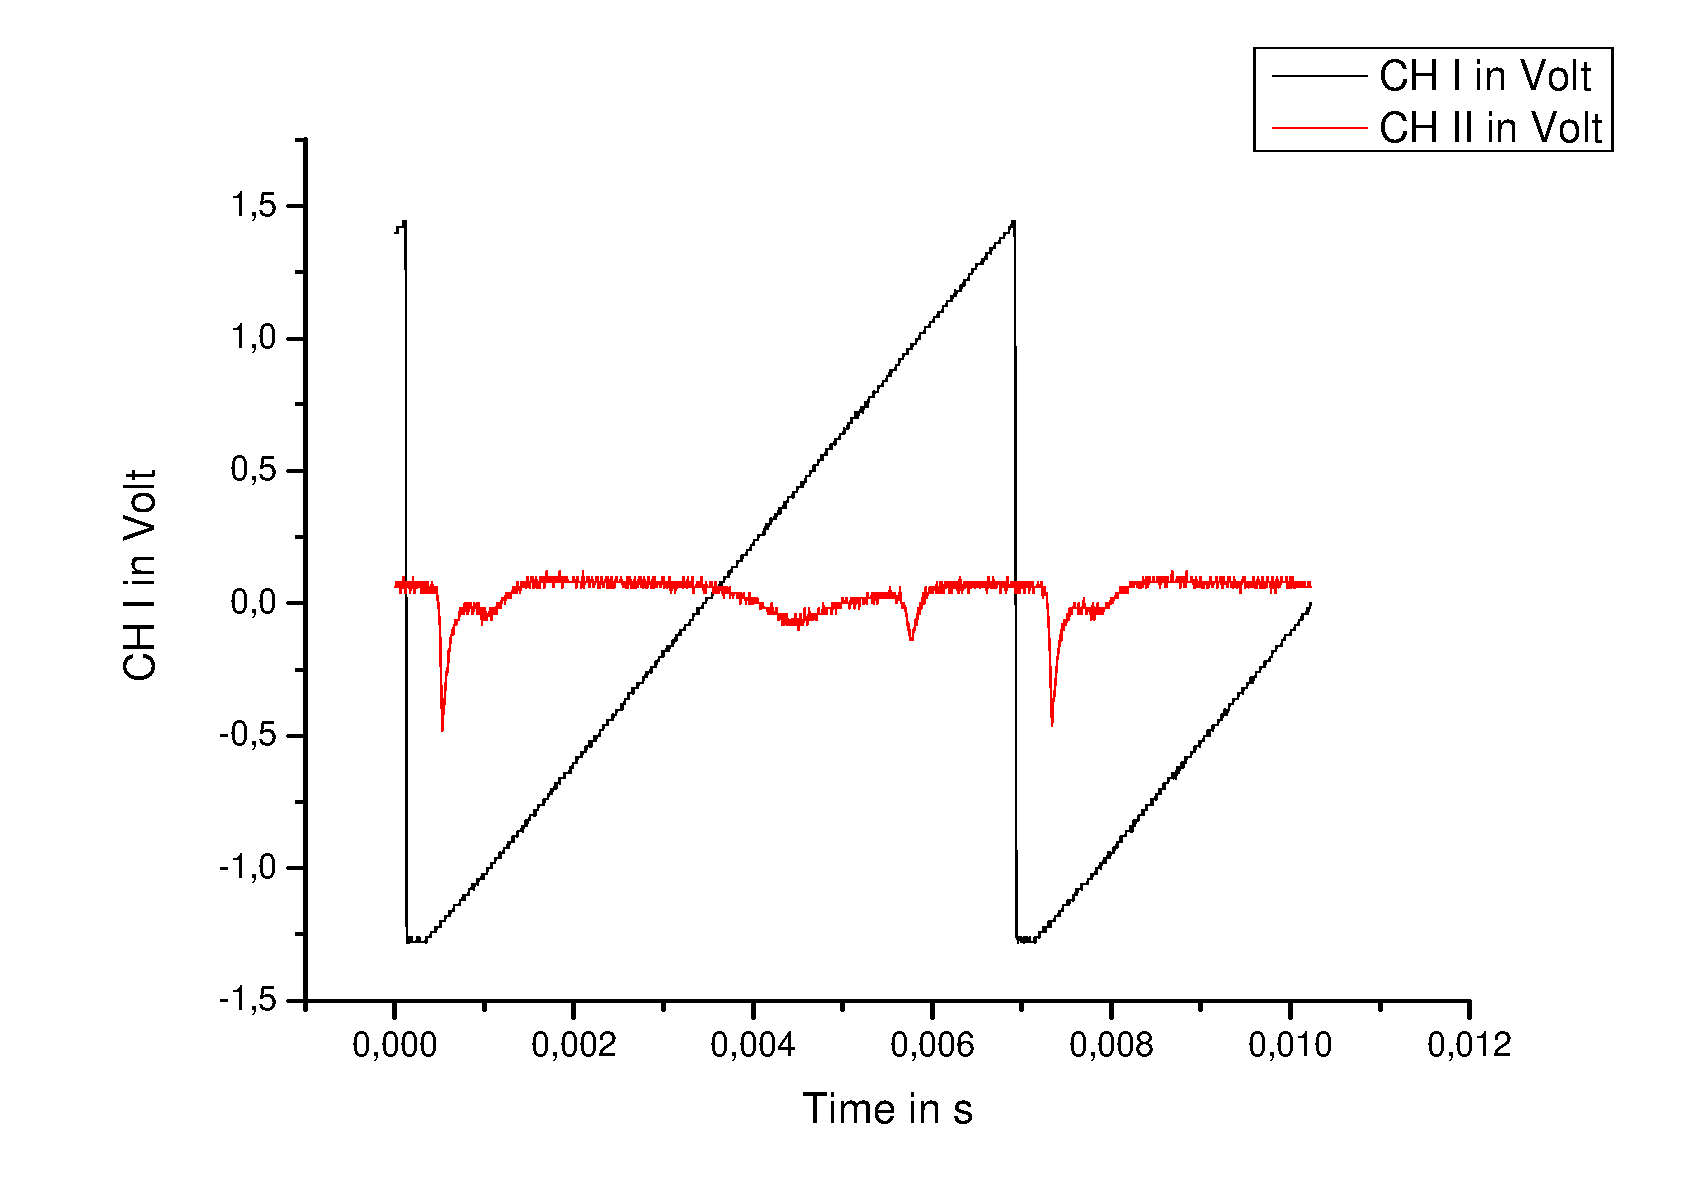
\includegraphics[width=1.1\textwidth]{Bilder/DR_SZ.pdf}
\end{column}
\end{columns}
\end{frame}

\begin{frame}{Prinzip der Doppelresonanz}
\begin{columns}
\begin{column}{3.5cm}
	\begin{figure}[H]
	\centering 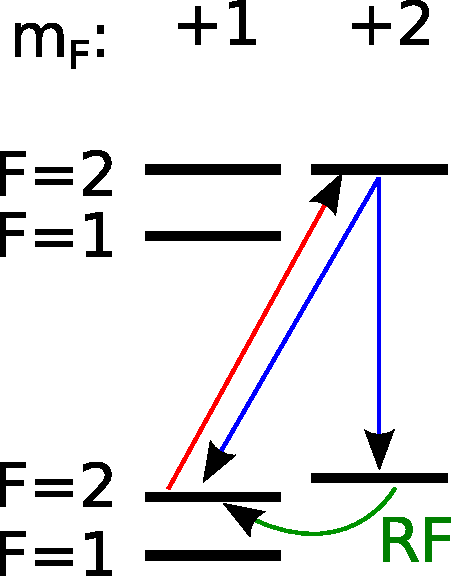
\includegraphics[width=\textwidth]{Bilder/OPRF.pdf}
	\end{figure}
\end{column}
\begin{column}{6.5cm}
\centering 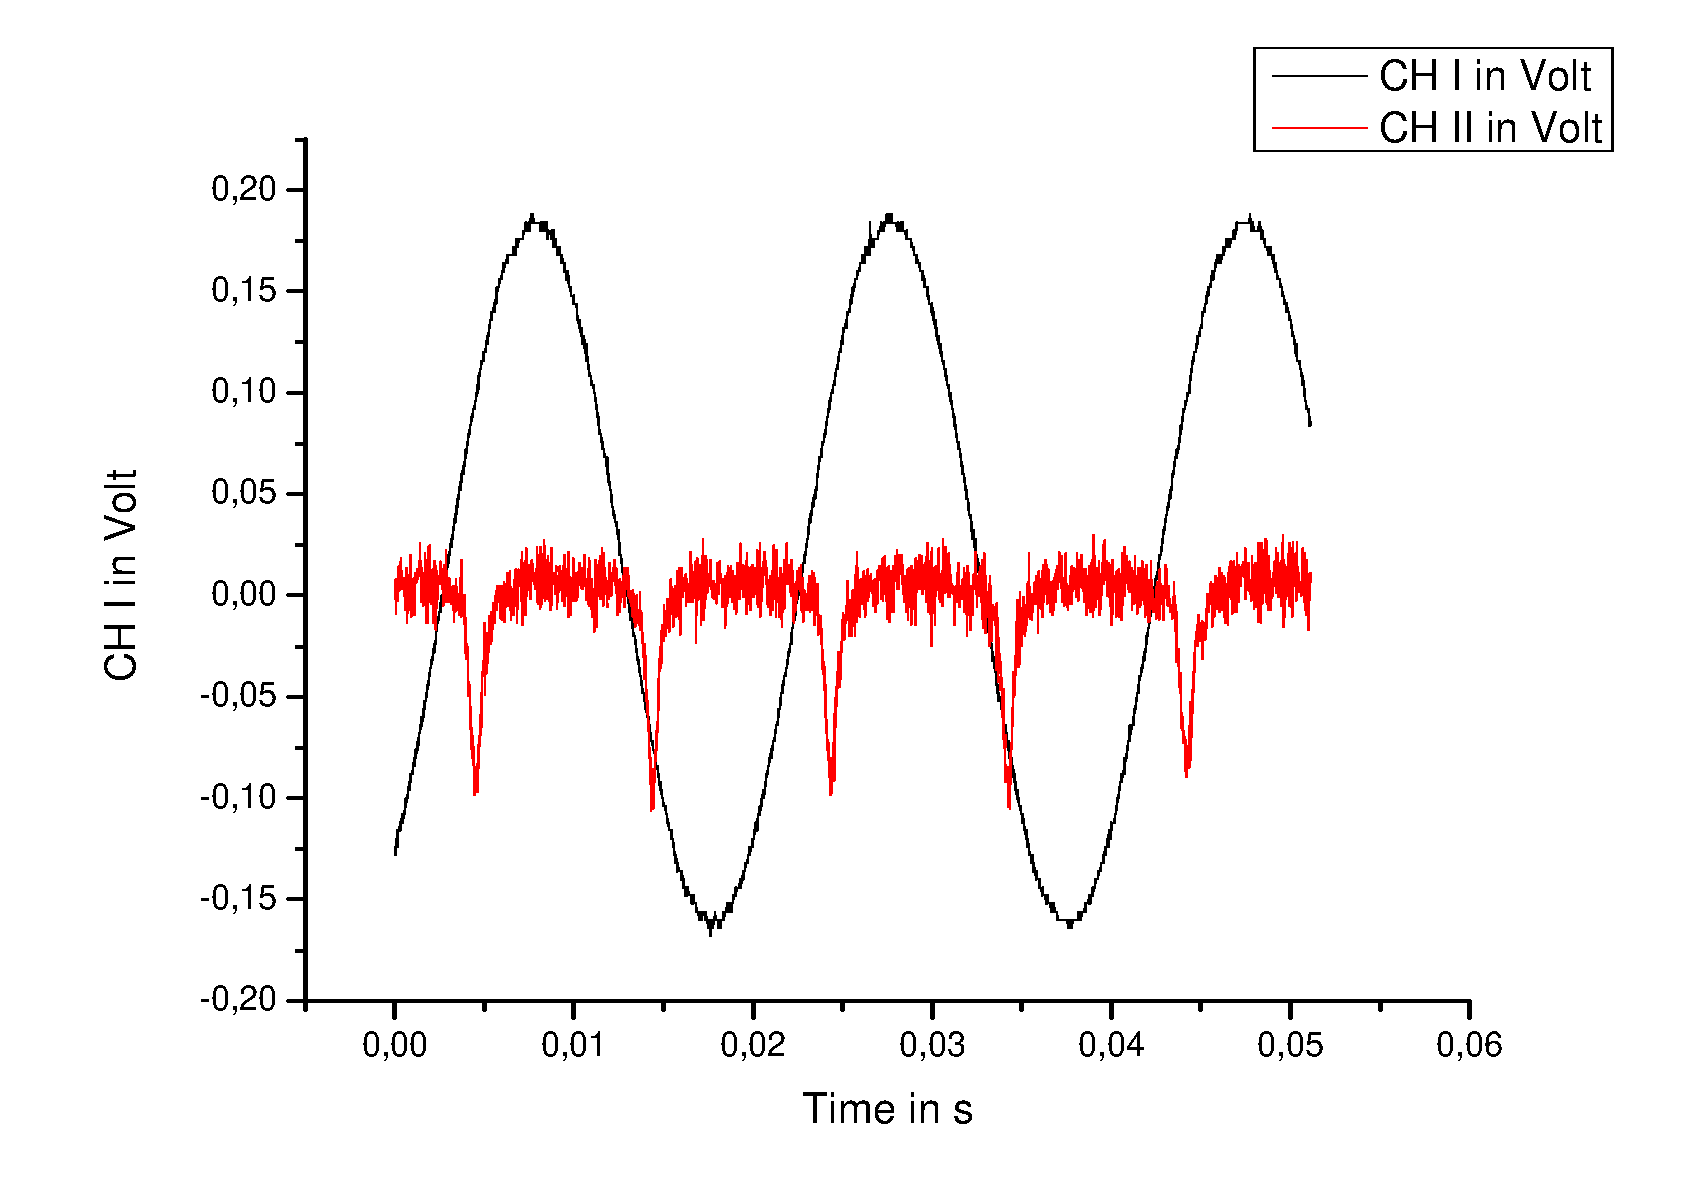
\includegraphics[width=1.1\textwidth]{Bilder/DR_sin.pdf}
\end{column}
\end{columns}
\end{frame}


\subsection{Resultate}
\begin{frame}{Messergebnisse}
\begin{block}{Resonanzfrequenzen des Lasers} %mit dem Sägezahn
$$I_1^L = (65.4 \pm 0.2)\ mA$$
$$I_2^L = (64.9 \pm 0.2)\ mA$$
\end{block}
\begin{exampleblock}{Erdmagnetfeld}
\begin{center}
\begin{tabular}[H]{c c c}
 & $B_{hor}/\mu T$ & $B_{vert}/\mu T$ \\ \hline
für $I_1^L$ & $9.19 \pm 1.1$ & $38.08 \pm 2.38$\\
für $I_2^L$& $8.39 \pm 1.1$ & $39.98 \pm 2.38$\\
Theorie & $20.9$ & $42.9$\\
St.-Abw. & 11, 12 & 3, 2\\
\end{tabular}
\end{center}
\end{exampleblock}
\end{frame}

\begin{frame}{Neuausrichtung des Tisches in Nord-Süd-Richtung}
\begin{center}
\centering 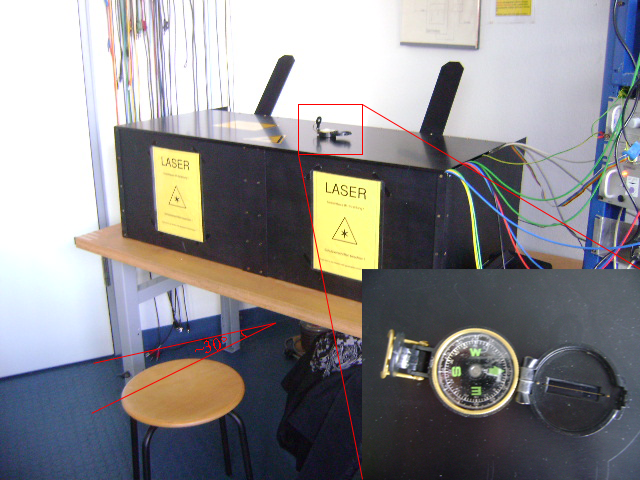
\includegraphics[width=0.8\textwidth]{Bilder/Nordsued.png}
\end{center}
\end{frame}

\begin{frame}{Neue Messergebnisse}
\begin{exampleblock}{Erdmagnetfeld}
\begin{center}
\begin{tabular}[H]{c c c}
			& $B_{hor}/\mu T$	& $B_{vert}/\mu T$ \\ \hline
für $I_1^L$	& $12.38 \pm 1.13$ 	& $38.56 \pm 2.38$\\
für $I_2^L$	& $12.38 \pm 1.13$ 	& $39.51 \pm 2.38$\\
Theorie 		& $20.9$ 			& $42.9$\\
St.-Abw. 		& 8				& 2\\
\end{tabular}
\end{center}
\end{exampleblock}
\end{frame}

\begin{frame}{Bestimmung des Kernspins}

$$E_{RF} = h\nu_{RF} = \frac{\mu_BB}{I+1/2} = E_{Zeeman}$$

$$\Rightarrow I = \frac{\mu_BB}{h\nu_{RF}}-\frac{1}{2} $$\\



Ergebnisse:\\

\begin{tabular}{| c c c c c c |} \hline
			& Isotop		& Kernspin	& Theorie	&	Fehler	& St.-Abw.\\ \hline
für $I_1^L$	& $^{87}Rb$	& $1.39\pm0.02$&	1.5	&	7.3\%	& 6\\
für $I_2^L$	& $^{85}Rb$	& $2.42\pm0.01$ &	2.5	&	3.2\%	& 8\\ \hline
\end{tabular}
\end{frame}

\section{Spinpräzession}
\begin{frame}
\begin{center}
\centering {\LARGE Spinpräzession}
\end{center}
\end{frame}

\subsection{Theorie}

\begin{frame}{Die Spinpräzession}
\centering 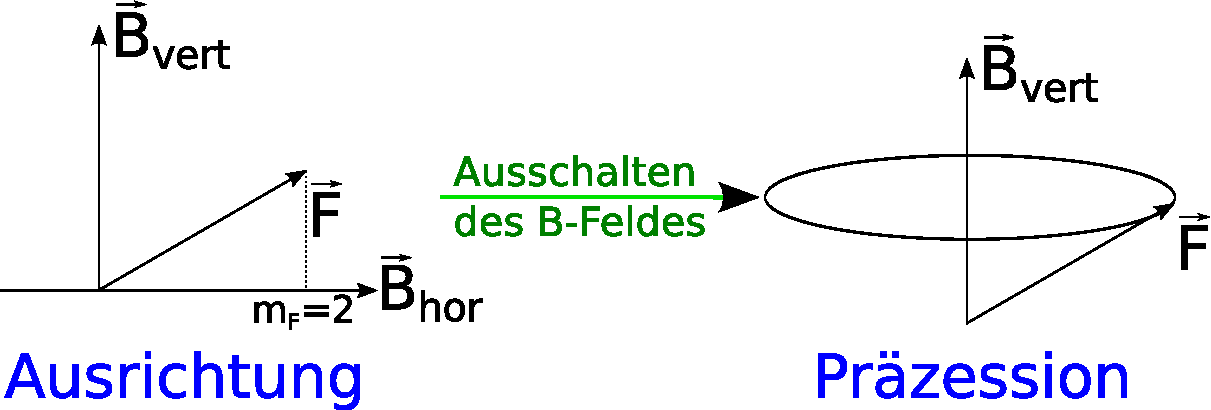
\includegraphics[width=\textwidth]{Bilder/praez.pdf}
\end{frame}

\subsection{Messung}
\begin{frame}{Beispiel einer Messung}
\centering 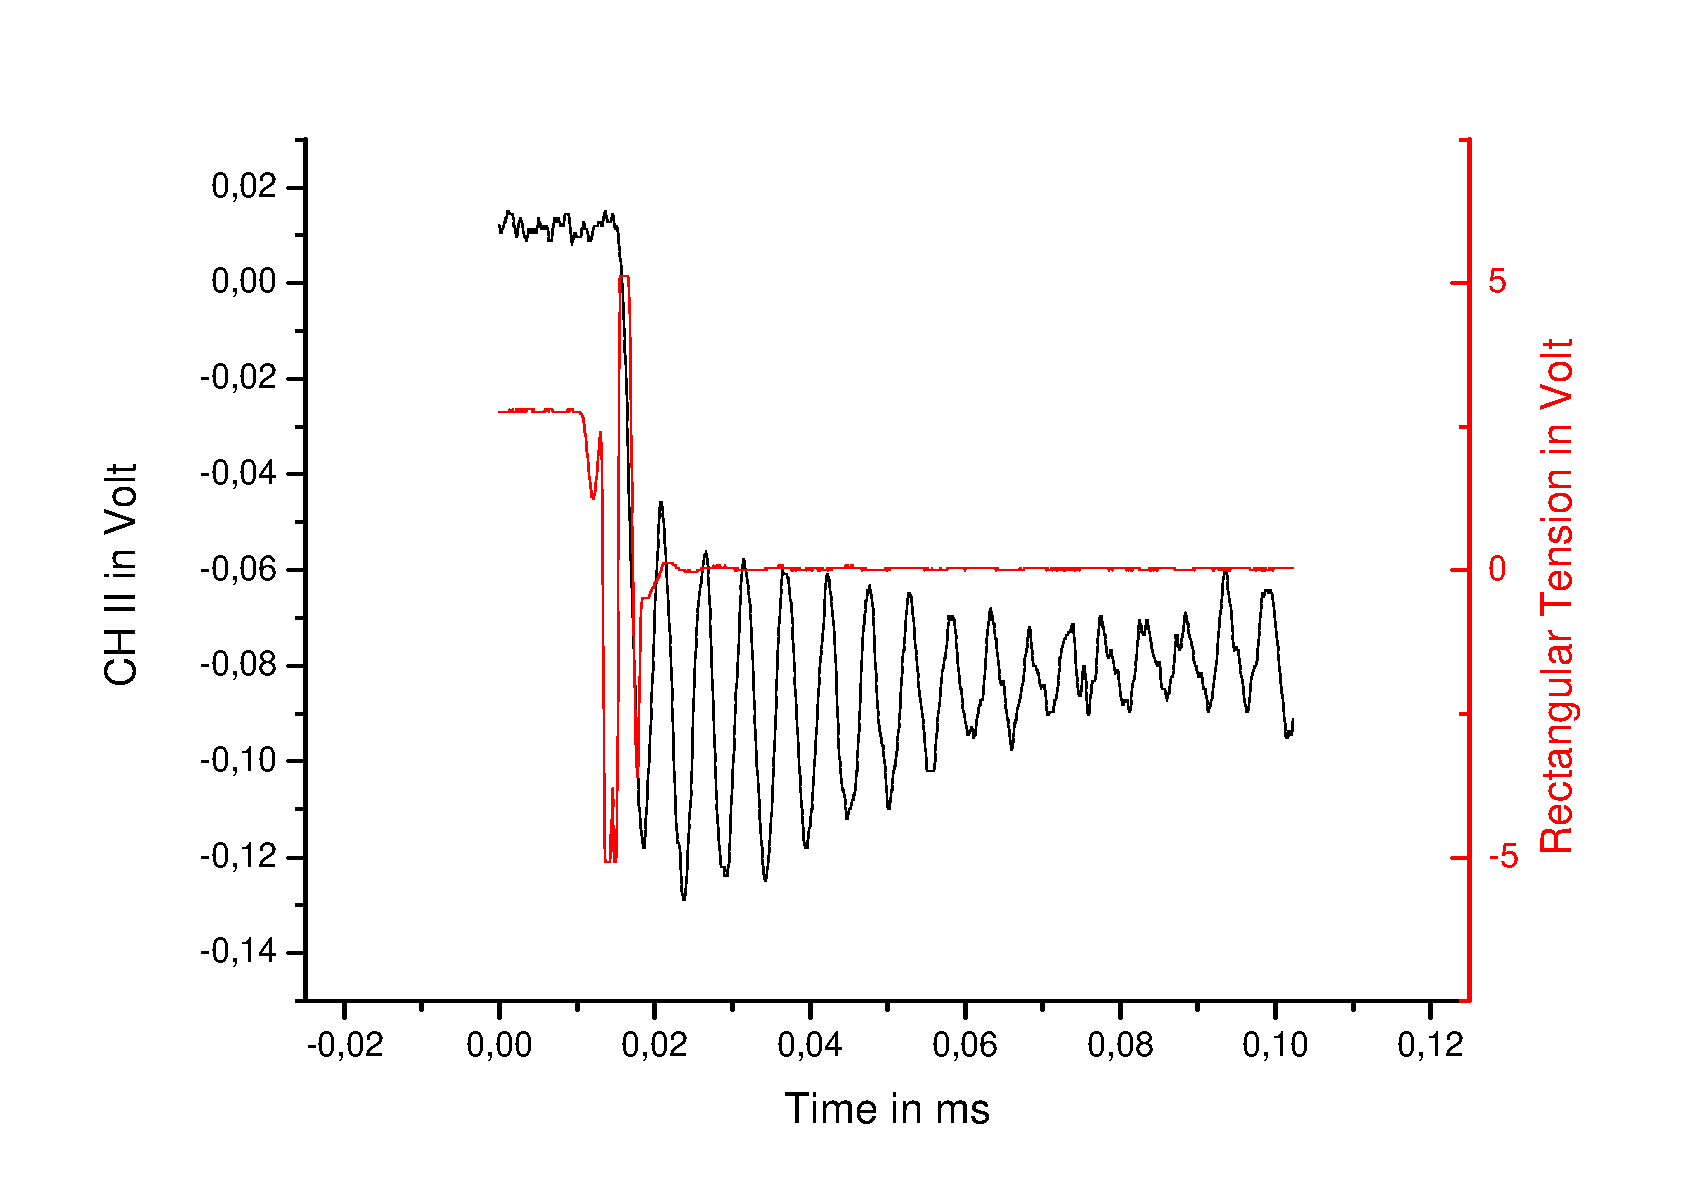
\includegraphics[width=0.9\textwidth]{Bilder/Spinpr.pdf}
\end{frame}

\begin{frame}{Messergebnisse}
Vetikales Erdmagnetfeld:

$$ B_{vert} = \frac{h\nu_{osz}}{\mu_BB} $$

\pause Ergebnis: $$\bar\nu_{osz} = (189.44 \pm 0.79)\ kHz$$

$$\Rightarrow\ \ \boxed{B_{vert} = (40.60 \pm 0.17)\ \mu T}$$ 

Theorie: 42.9 $\mu T$, somit 5\% bzw 14 Standard-Abweichungen
\end{frame}

\begin{frame}{Messung mit anderen vertikalen Feldern}
\centering 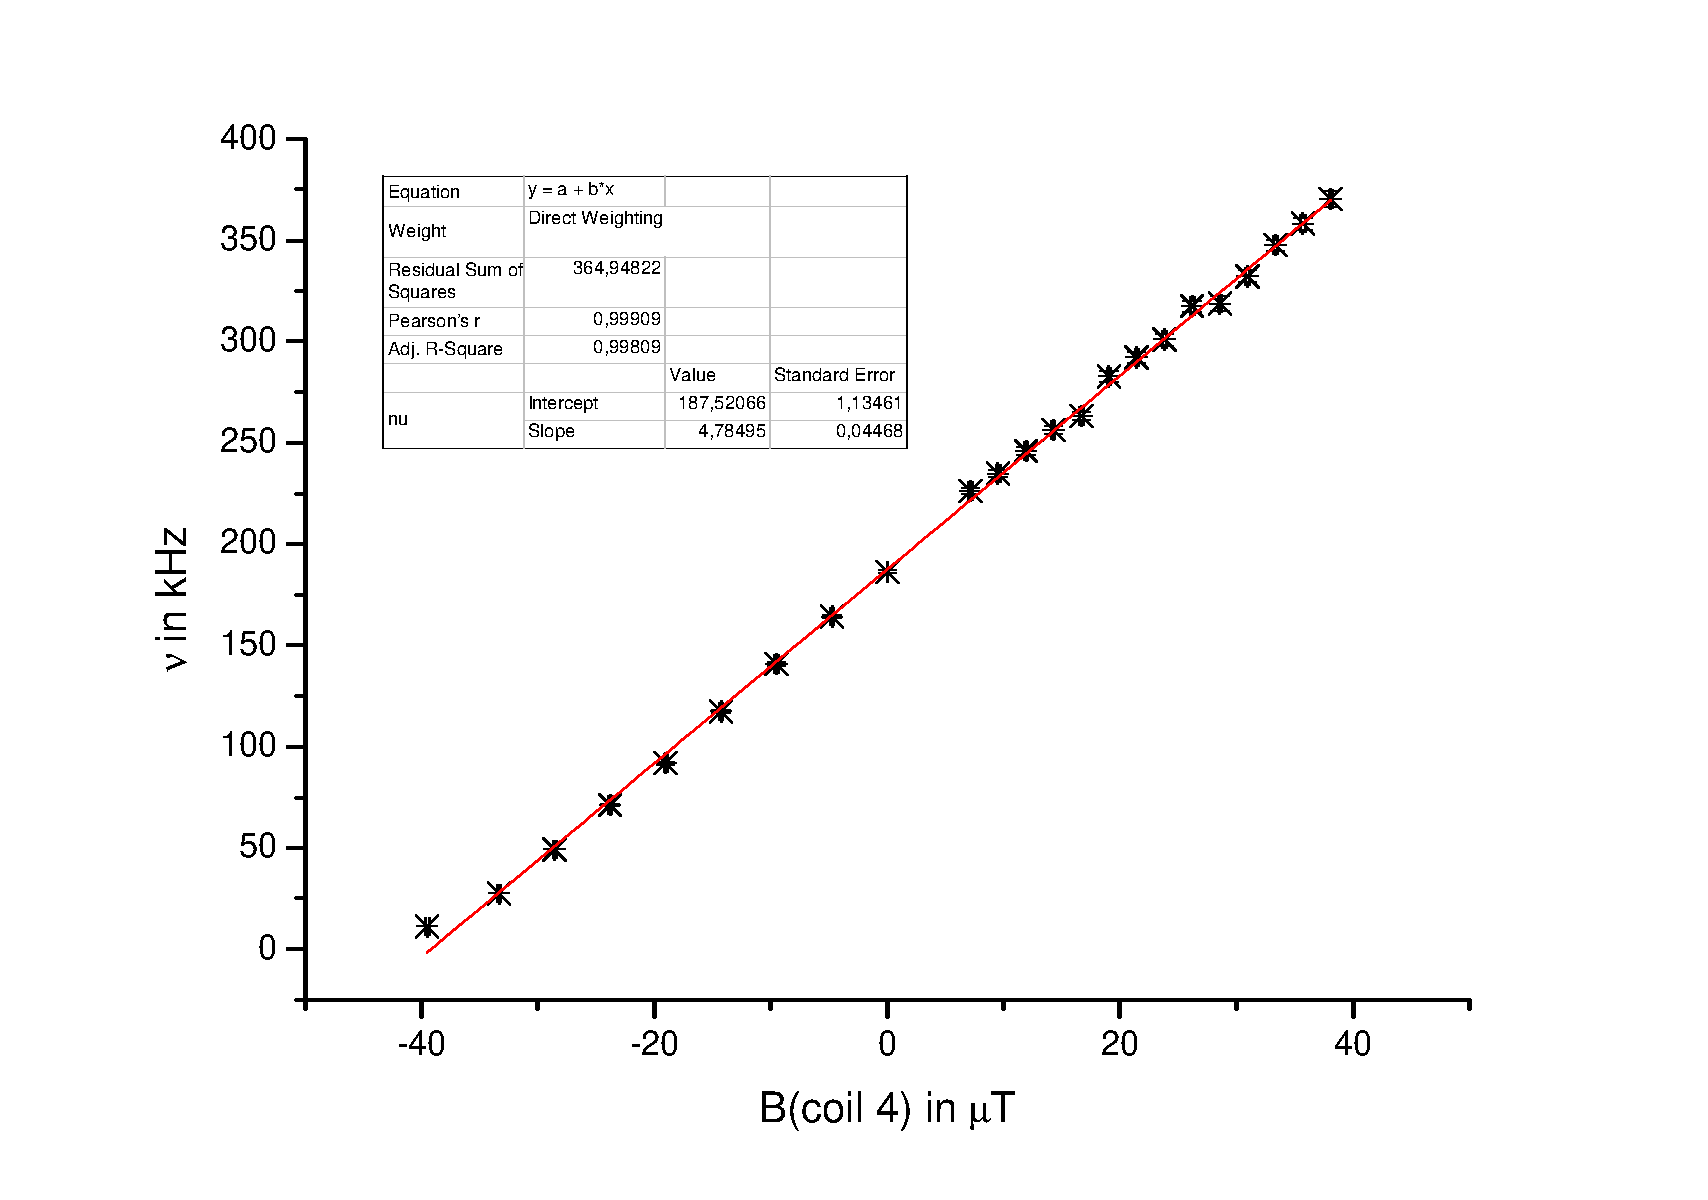
\includegraphics[width=0.75\textwidth]{Bilder/praezfeld.pdf}
$$\text{Zusammenhang: } \nu_{osz} = (4.78\pm0.04)B_{vert} \frac{kHz}{\mu T} + (187.52 \pm 1.13)kHz$$
\end{frame}

\section{Relaxationszeit}
\begin{frame}
\begin{center}
\centering {\LARGE Die Relaxationszeit}
\end{center}
\end{frame}

\subsection{Theorie}
\begin{frame}{Theorie}
Depolarisation durch:
\begin{itemize}
\item Stöße an der Zellwand
\item Stöße am Puffergas
\item Spinaustausch
\end{itemize}

Differentialgleichung des Pumpprozesses:
 $$\frac{dn}{dt} = \left(\frac{dn}{dt}\right)_{pump} + \left(\frac{dn}{dt}\right)_{relax} = \frac{N_{tot}-n}{T_P} - \frac{n}{T_R}$$ %erklären der Komponenten
\end{frame}

\begin{frame}{Theorie}
Lösung der DGL:

$$n(t) = n_{max}(1-\exp(-t/\tau))$$

mit

$$\frac{1}{\tau} = \frac{1}{T_{pump}} + \frac{1}{T_{relax}}$$ %einzelllösungen

und $$T_{pump} \sim I^{-1}$$ %also I-->0 => 1/TP-->0

\end{frame}

\subsection{Dehmelt}
\begin{frame}{Die Dehmelt-Methode}
\begin{center}
\centering 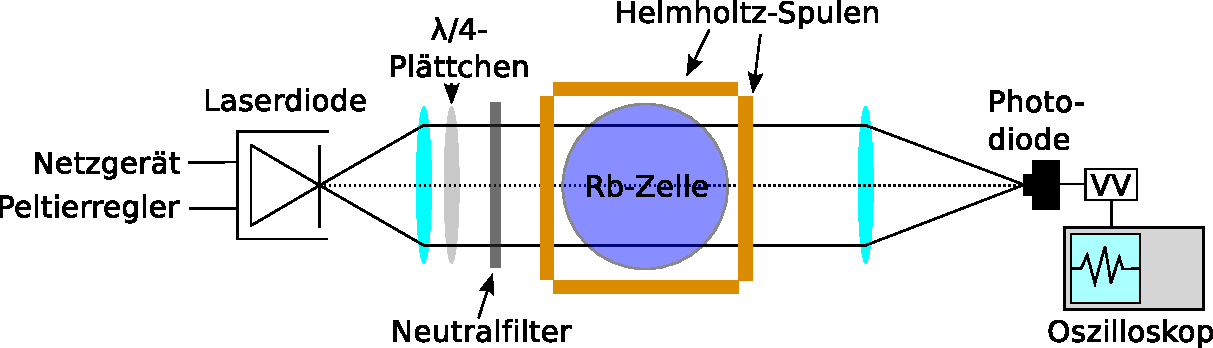
\includegraphics[width=\textwidth]{Bilder/ABDehmelt.pdf}
\end{center}
\end{frame}

\begin{frame}{Beispielmessung}
\begin{center}
\centering 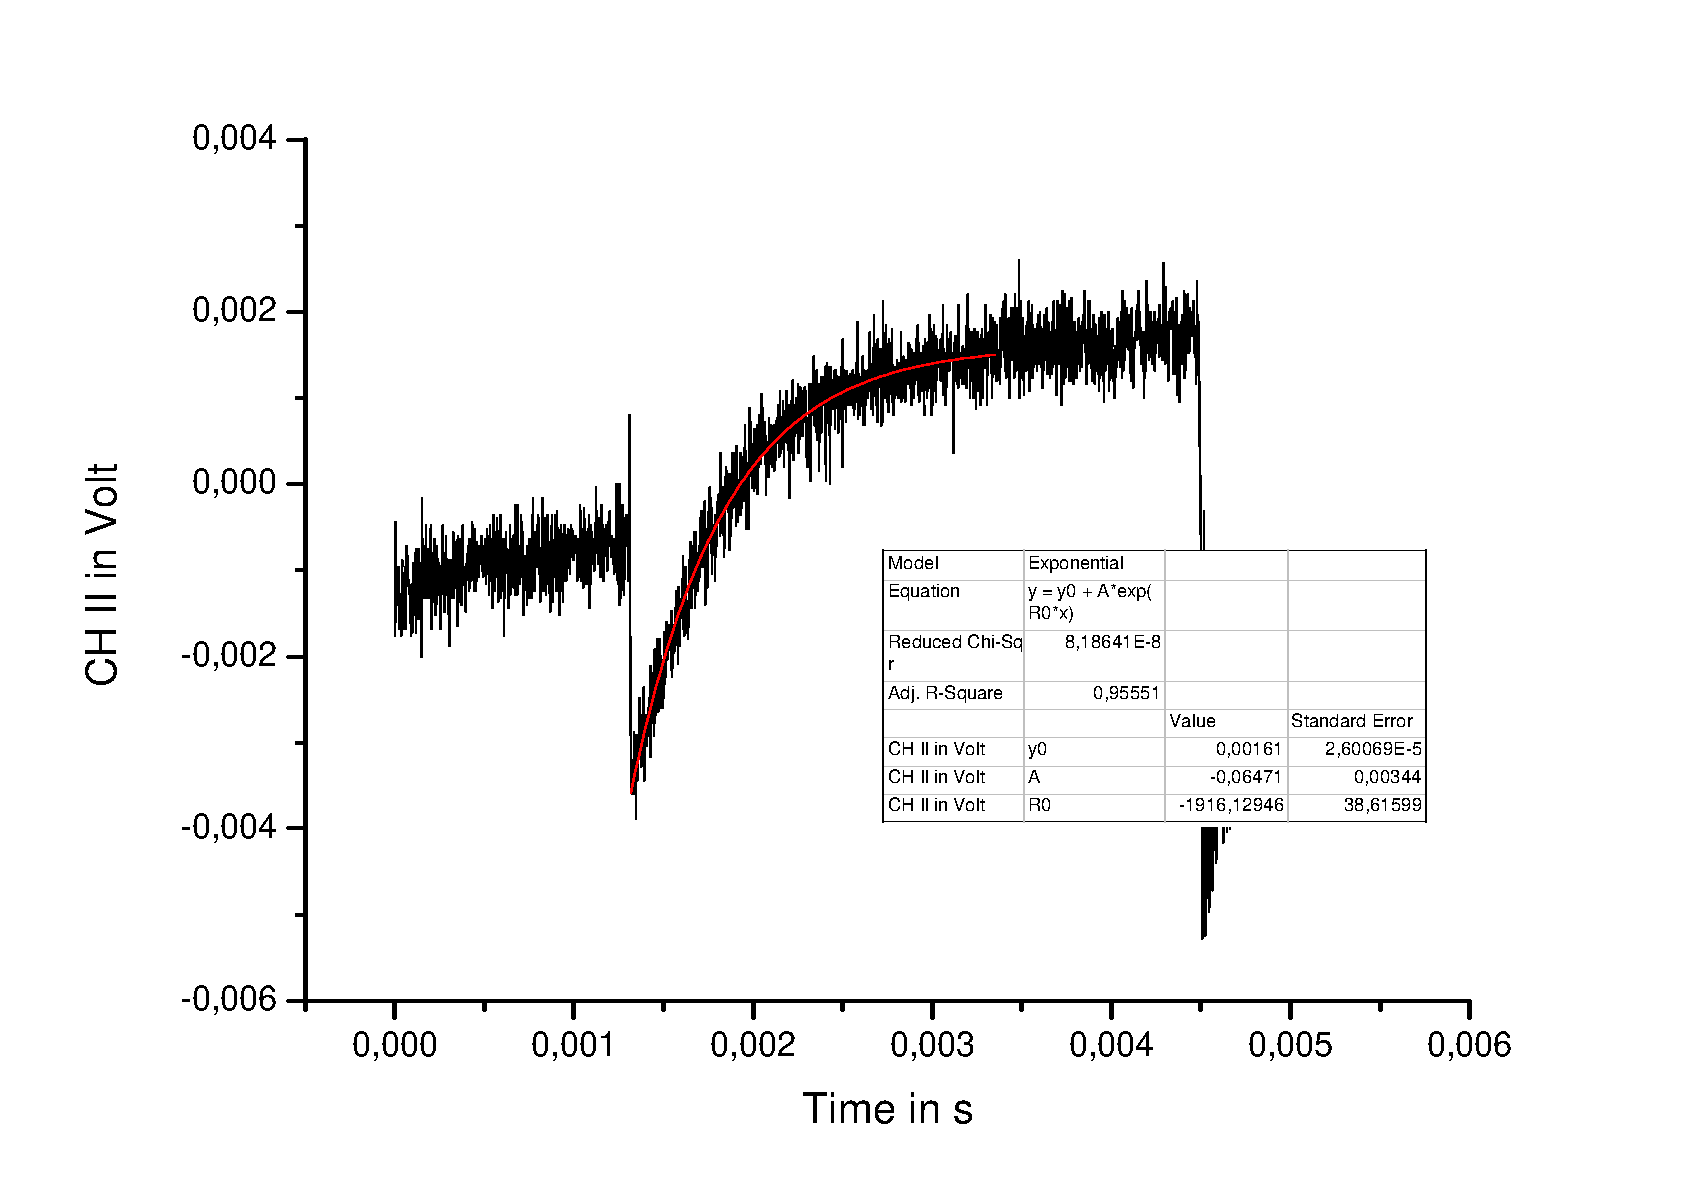
\includegraphics[width=0.9\textwidth]{Bilder/DehmeltBsp.pdf}
\end{center}
\end{frame}

\begin{frame}{Ergebnis}
\begin{center}
\centering 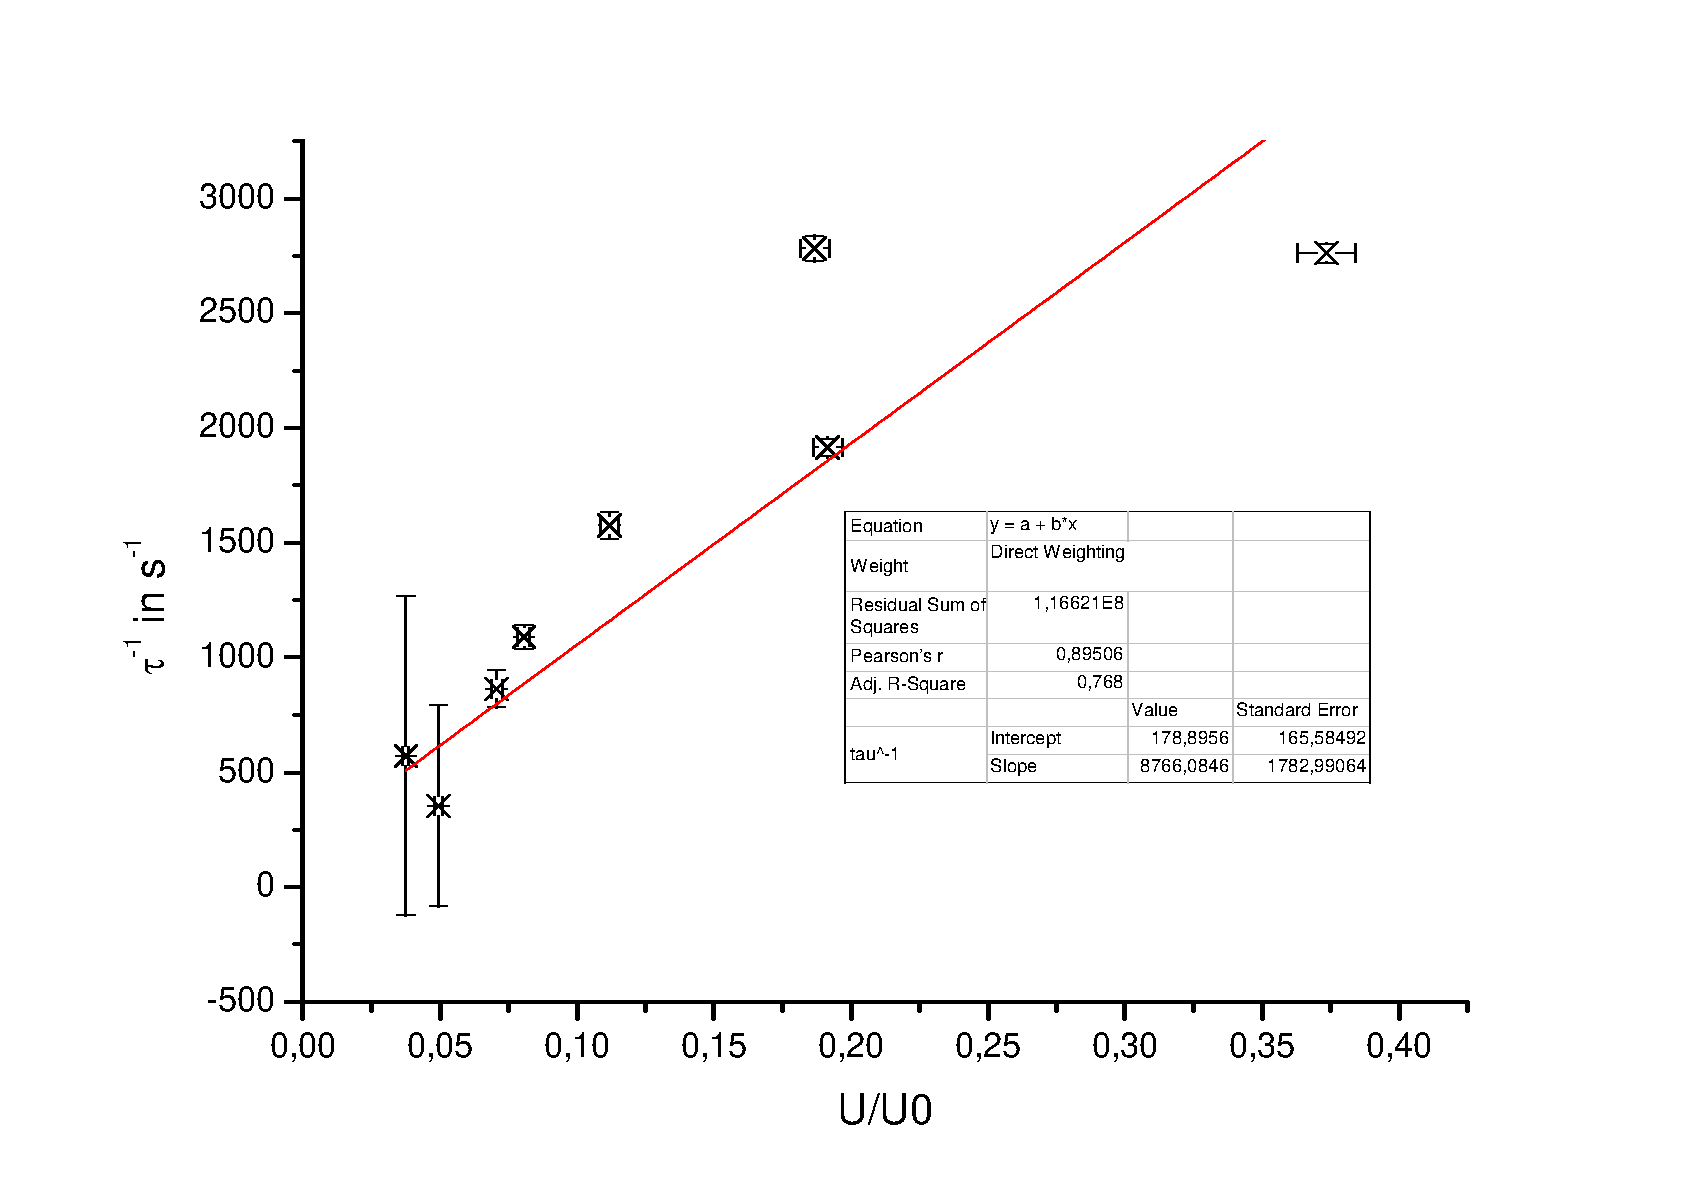
\includegraphics[width=0.9\textwidth]{Bilder/Dehmelt.pdf}
\end{center}
\end{frame}

\begin{frame}{Ergebnis}
$$\frac{U}{U_0} \sim I \to 0 \ \ \Rightarrow \ \ \frac{1}{T_{pump}} \to 0$$
Somit gilt $$\tau(0) = T_{relax}$$
Ergebnis durch Achsenabschnitt:

$$ T_{relax} = (5.590 \pm 5.174)\ ms$$ %diskussion, korrekter bereich jedoch großer fehler => föhnen

\end{frame}

\subsection{Franzen}
\begin{frame}{Die Franzen-Methode}
\begin{center}
\centering 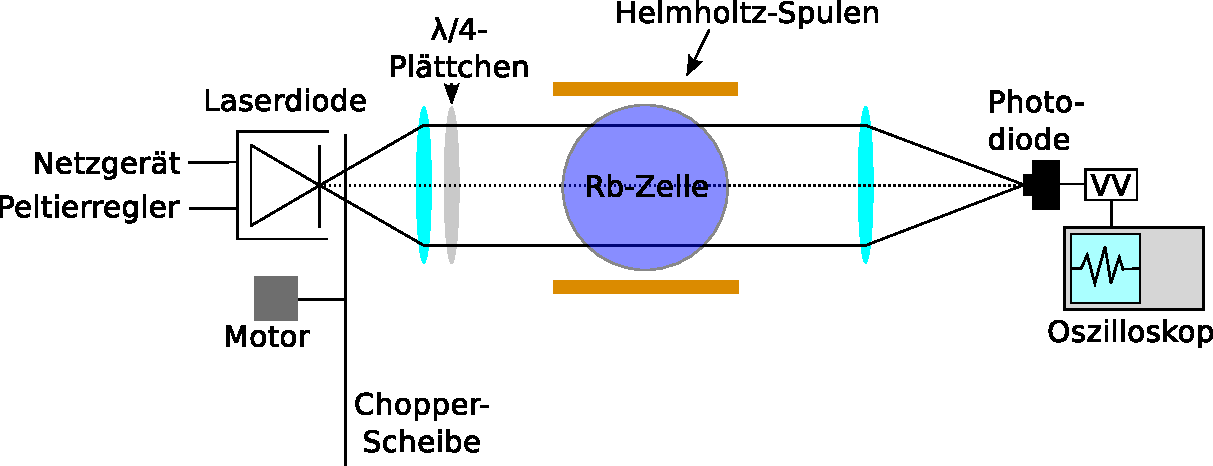
\includegraphics[width=\textwidth]{Bilder/ABFranzen.pdf}

\centering 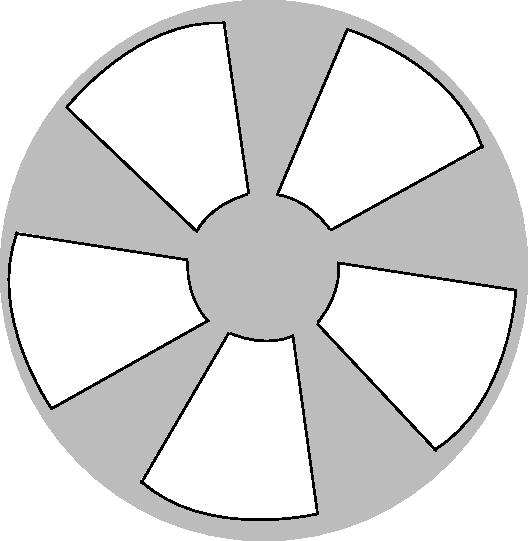
\includegraphics[width=0.18\textwidth]{Bilder/chopper.pdf}
\end{center}
\end{frame}

\begin{frame}{Beispielmessung}
\begin{center}
\centering 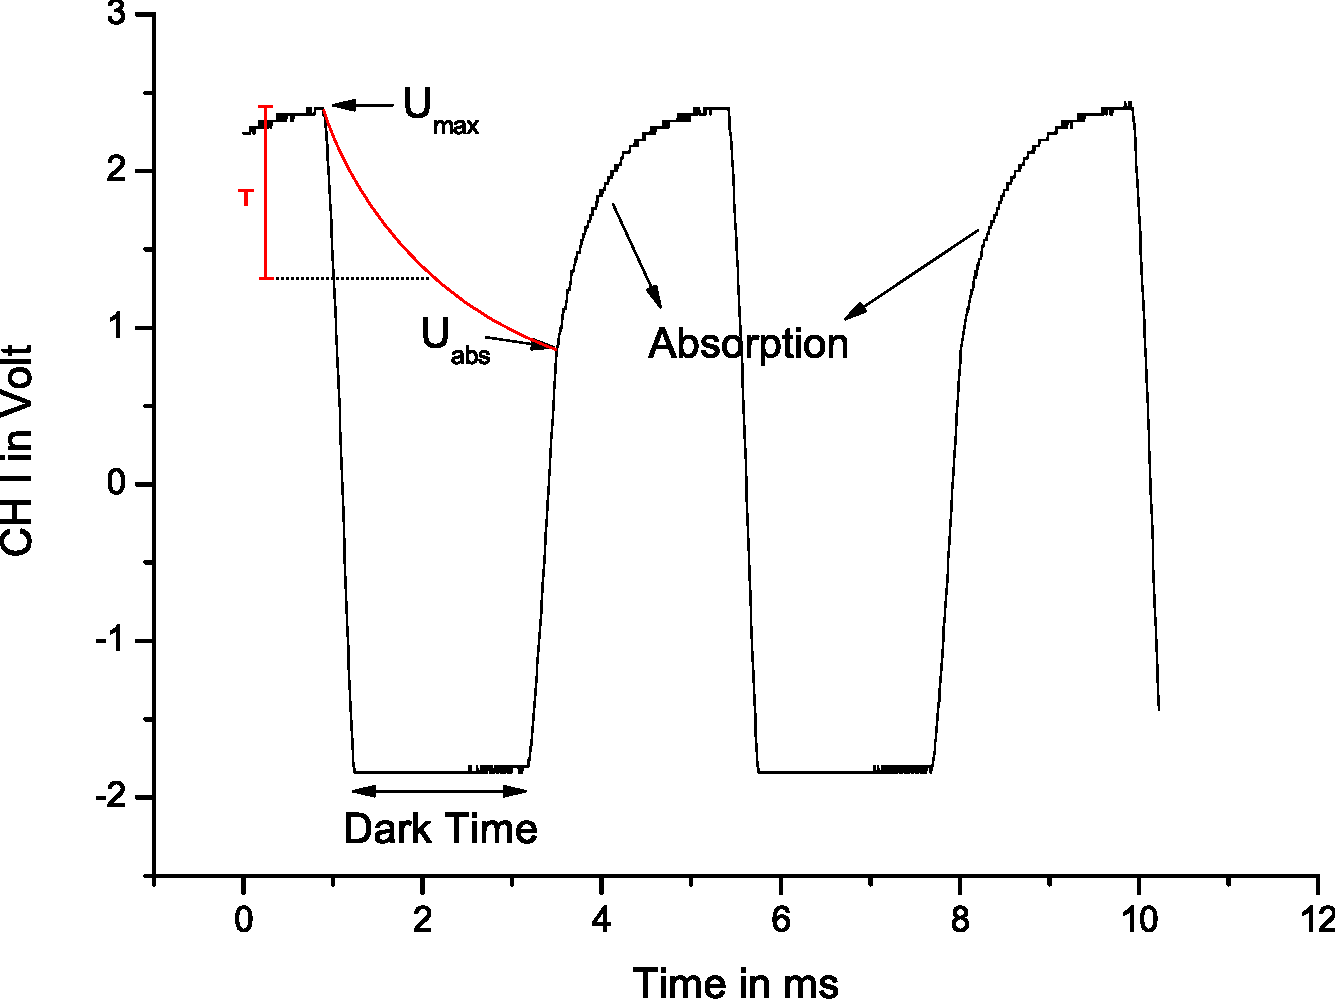
\includegraphics[width=0.8\textwidth]{Bilder/FranzenBsp.pdf}
\end{center}
\end{frame}

\begin{frame}{Ergebnis}
\begin{center}
\centering 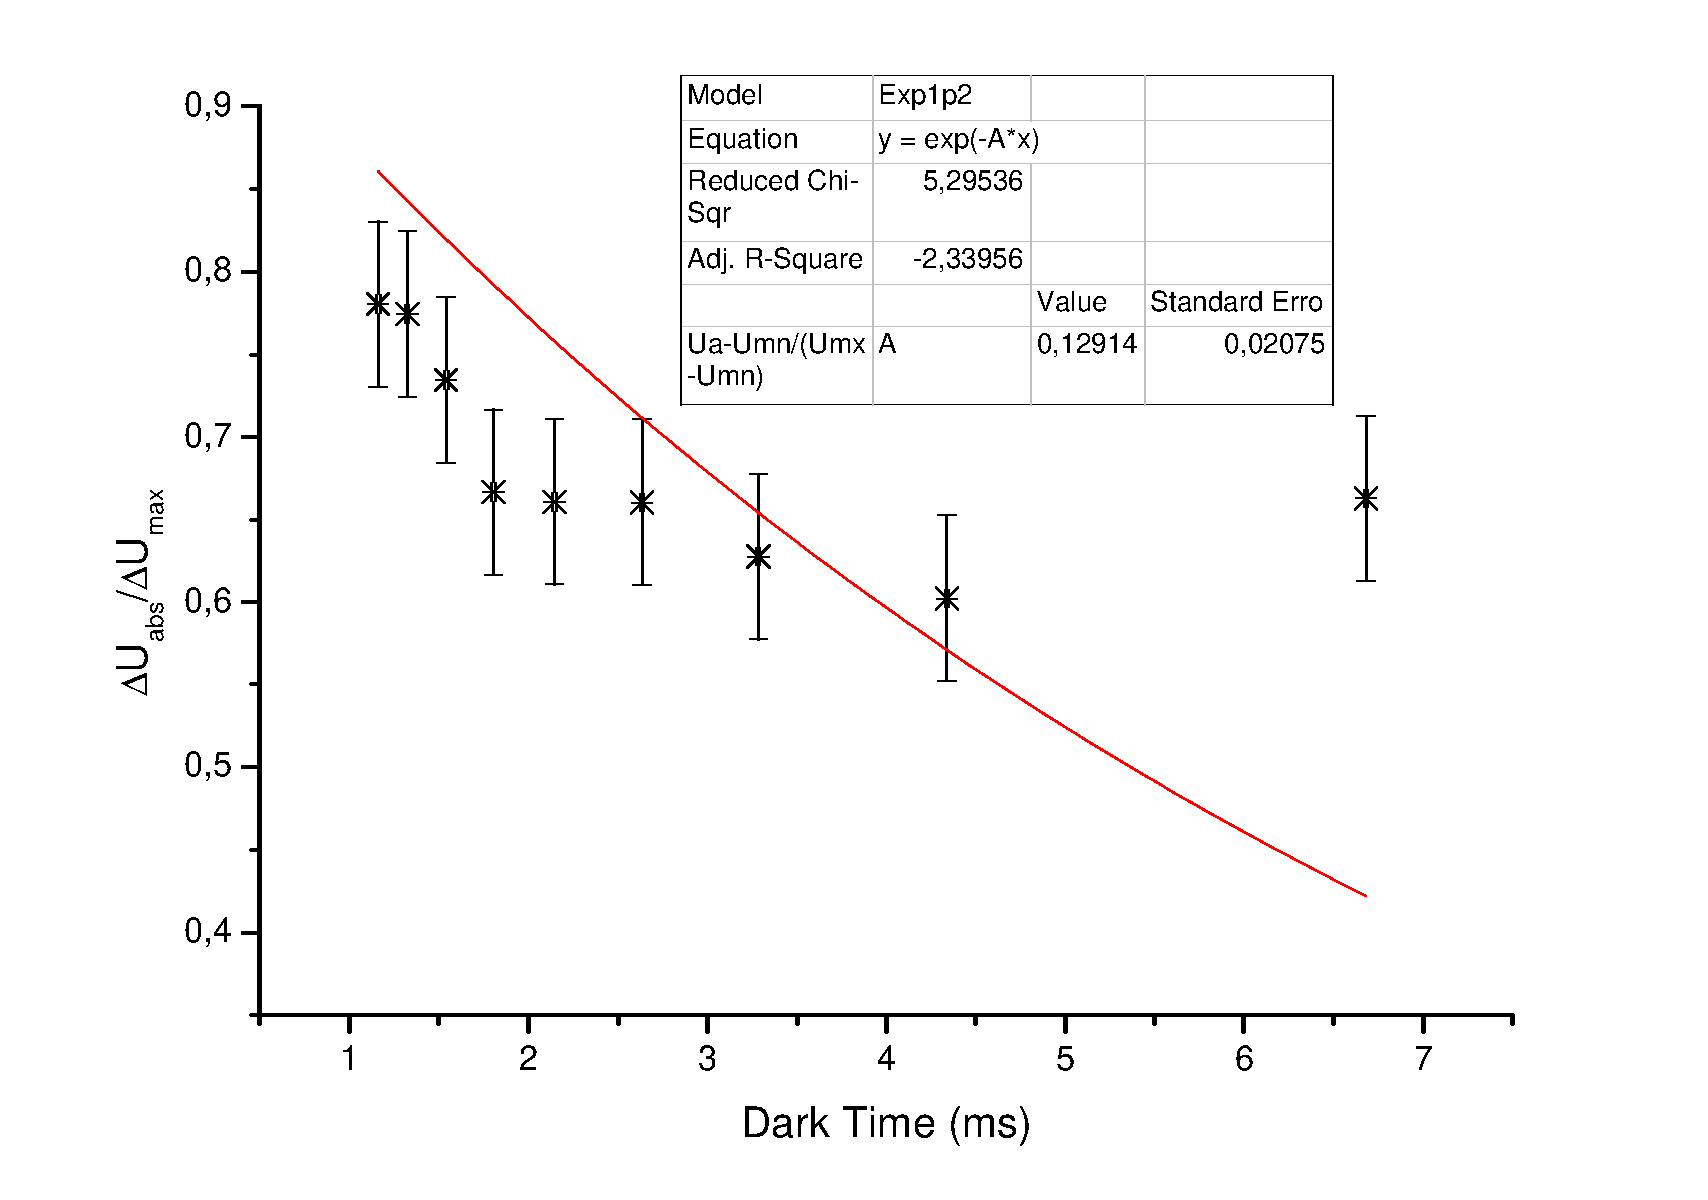
\includegraphics[width=0.9\textwidth]{Bilder/Franzen.pdf}
\end{center}
\end{frame}

\begin{frame}{Ergebnis}
$$I(\Delta t) = I_{min} + (I_{max}-I_{min})\exp\left(-\frac{\Delta t}{T_{relax}}\right)$$ %annahme dass U~I
$$\frac{U_{abs}-U_{min}}{U_{max}-U_{min}} = \exp\left(-\frac{\Delta t}{T_{relax}}\right)$$

Somit:

$$T_{relax} = (7.744 \pm 1.244)\ ms$$ %diskussion korrekter fehlerbereich

\end{frame}


\subsection{Ergebnisse}
\begin{frame}{Vergleich der Relaxationszeiten}
$$T_{Dehmelt} = (5.590 \pm 5.174)\ ms$$
$$T_{Franzen} = (7.744 \pm 1.244)\ ms$$

Gewichtetes Mittel:

$$\boxed{T_{relax} = (7.626 \pm 1.210)\ ms} $$

\pause $$T_{theo} = \text{einige ms, \ \ \ Staatsexamensarbeit: 6.5 ms} \dots Temperatur?$$

\end{frame}

\section{Fazit}
\begin{frame}{Fazit}
\end{frame}

\end{document}
